\chapter{RANCANGAN DAN IMPLEMENTASI SISTEM}
% DOCX block 471
Kerja praktik di Divisi Maintenance PT XYZ berlangsung pada periode 1 Juli sampai dengan 31 Desember 2026. Kegiatan Muhammad Fandy Anggriawan berfokus pada sistem monitoring mesin cutting, sedangkan Muhammad Fadhil Abdillah mengembangkan monitoring panel listrik. Bab ini menjelaskan kebutuhan, perangkat, aplikasi, integrasi data, dan evaluasi kedua proyek. Pembahasan diawali dengan observasi dan pengembangan sistem mesin cutting, dilanjutkan dengan sistem panel di area Power Room, integrasi dashboard, serta evaluasi kedua sistem. Bagian akhir menguraikan dokumentasi pekerjaan, kontribusi penulis, dan korelasi kegiatan dengan mata kuliah.

% DOCX block 472
\section{Bidang Kegiatan Kerja Praktik}

% DOCX block 473
\subsection{Pengantar}

% DOCX block 474
Sistem monitoring membaca kondisi mesin, menampilkan hasilnya pada HMI, menyimpan riwayat, dan mengirim data ke dashboard server. Pekerjaan mencakup penyambungan sensor, pembuatan aplikasi, serta pengaturan alarm. Implementasi mesin cutting telah selesai dengan konfigurasi yang disesuaikan untuk perangkat pada masing-masing mesin.

% DOCX block 475
\subsection{Observasi Proses Kerja dan Identifikasi Permasalahan}

% DOCX block 476
Mesin cutting digunakan pada tahap pengolahan kabel dalam produksi wiring harness. Sistem memantau suhu motor, arus tiga fasa, tekanan udara, dan laju aliran udara sesuai konfigurasi mesin. Pengguna dapat melihat nilai pengukuran di dekat mesin dan membuka kembali riwayatnya.

% DOCX block 477
Perangkat ukur mempunyai keluaran sinyal yang berbeda. Sistem harus mengubah sinyal tersebut menjadi nilai pengukuran, menampilkannya pada HMI, menyimpannya, lalu mengirimkannya ke server. Program juga harus mengenali pembacaan yang gagal dan membedakan data terbaru dari riwayat pengukuran.

% DOCX block 478
Untuk memenuhi kebutuhan tersebut, perangkat ukur dihubungkan melalui Modbus RTU. HMI menampilkan data, SQLite menyimpan riwayat, dan MQTT mengirimkannya ke server. Fungsi alarm dan pemeriksaan kartu RFID digunakan untuk menangani peringatan.

% DOCX block 479
\subsection{Analisis Kebutuhan Integrasi}

% DOCX block 480
Integrasi sistem mempertimbangkan perbedaan karakteristik sinyal dari perangkat pengukuran. Suhu motor dibaca menggunakan sensor PT100 melalui konverter RTD--RS485. Tiga transduser arus satu fasa, sensor tekanan, dan sensor aliran udara dihubungkan ke modul masukan analog untuk mengubah sinyal pengukuran menjadi data yang dapat dibaca melalui Modbus RTU.

% DOCX block 481
Raspberry Pi membaca data dari konverter RTD dan modul masukan analog, lalu mengolah, menampilkan, dan menyimpannya. Pengaturan pembacaan mengikuti perangkat yang digunakan pada setiap mesin cutting.

% DOCX block 482
\subsection{Analisis Perangkat atau Sistem yang Digunakan}

% DOCX block 483
Perangkat utama sistem terdiri atas Raspberry Pi, satu konverter Waveshare USB--RS485, sensor PT100 beserta konverter RTD--RS485, tiga transduser arus satu fasa, modul masukan analog Waveshare, sensor tekanan SMC ISE30A-01-D, dan sensor aliran udara SMC PFMB7202-06-C. Touch Display 7 inci digunakan sebagai antarmuka fisik HMI. Perangkat pendukung meliputi pembaca RFID, relay, buzzer 24 VDC, serta catu daya 24 VDC dan 5 VDC. Fungsi platform Raspberry Pi dan modul masukan analog didukung oleh dokumentasi perangkat \citep{raspberrypi}, \citep{waveshare}.

% DOCX block 484
Jenis keluaran sensor menentukan cara penyambungannya. Kanal masukan, rentang konversi, alamat perangkat, dan port komunikasi diatur agar program mengetahui sumber serta satuan setiap nilai yang dibaca.

% DOCX block 485
\subsection{Alur Kerja Sistem Monitoring Mesin Cutting}

% DOCX block 486
Gambar~\ref{fig:draft-3-1} menunjukkan alur pembacaan sensor. PT100 terhubung ke konverter RTD--RS485. Tiga transduser arus satu fasa, sensor tekanan SMC ISE30A-01-D, dan sensor aliran SMC PFMB7202-06-C terhubung ke modul Waveshare. Transduser arus menghasilkan sinyal 4--20 mA DC atau 0--5 VDC sesuai unit yang terpasang. Sensor tekanan menghasilkan arus DC 4--20 mA, sedangkan sensor aliran menghasilkan tegangan 1--5 VDC. Konverter RTD dan modul Waveshare menyediakan hasil pembacaan melalui Modbus RTU.

% DOCX block 487
Satu konverter Waveshare USB--RS485 menghubungkan Raspberry Pi dengan konverter RTD--RS485 dan modul masukan analog Waveshare pada bus yang sama. Konverter RTD menggunakan slave ID 1, sedangkan Waveshare Modbus RTU Analog Input 8CH menggunakan slave ID 2. Aplikasi memilih perangkat yang dibaca melalui alamat tersebut. Hasilnya ditampilkan pada Touch Display 7 inci melalui DSI. Catu daya 24 VDC memasok perangkat pengukuran dan buzzer, sedangkan catu daya 5 VDC khusus untuk Raspberry Pi. Saat alarm aktif, Raspberry Pi mengendalikan relay melalui GPIO untuk menyambungkan suplai 24 VDC ke buzzer. Pembaca RFID mengirim identitas kartu teknisi untuk penanganan peringatan.

% DOCX block 488
\begin{figure}[htbp]
  \centering
  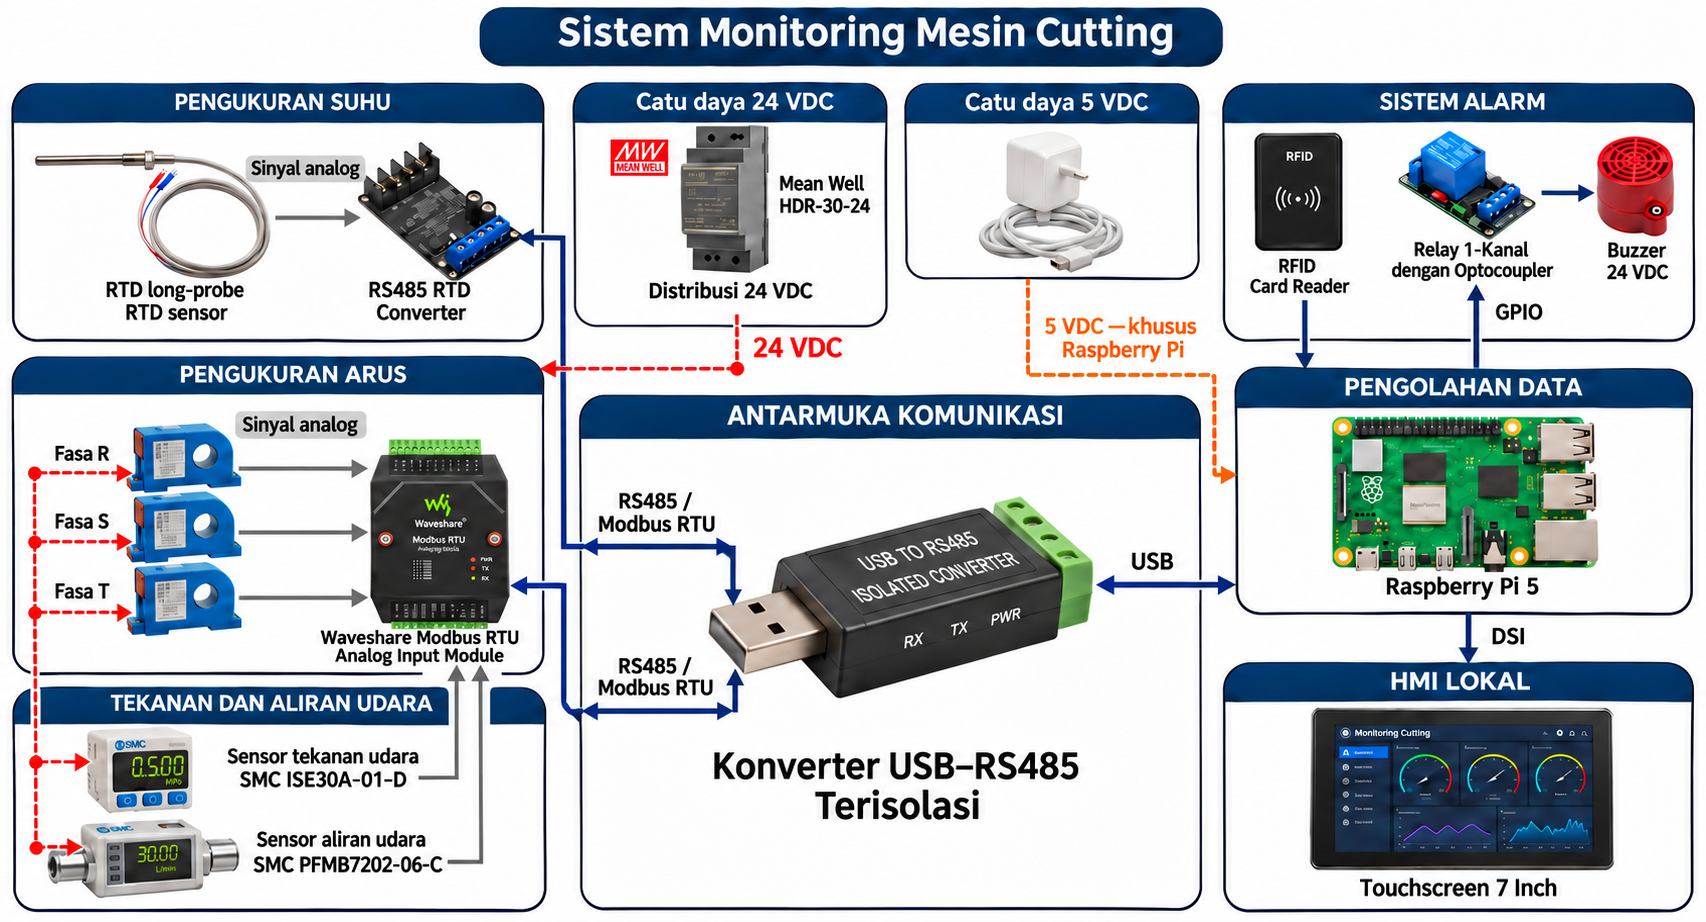
\includegraphics[width=\linewidth,keepaspectratio]{assets/gambar/gambar-4-01.png}
  \caption{Blok diagram sistem monitoring mesin cutting}
  \label{fig:draft-3-1}
\end{figure}

% DOCX block 489
\subsection{Pengembangan Sistem Monitoring Mesin Cutting}

% DOCX block 490
Perangkat lunak terdiri atas aplikasi HMI pada Raspberry Pi dan dashboard pada server. HMI menggunakan Python dan PyQt5 untuk membuat tampilan, pyqtgraph untuk grafik, serta minimalmodbus dan pyserial untuk membaca perangkat. SQLite menyimpan data pada mesin, sedangkan paho-mqtt mengirim pesan melalui MQTT. Dashboard menggunakan Django, HTML, CSS, JavaScript, dan Chart.js. Raspberry Pi menangani pembacaan serta peringatan di dekat mesin, sementara server menyediakan pemantauan terpusat.

% DOCX block 491
Aplikasi HMI dapat diatur sesuai perangkat setiap mesin cutting. Pengaturannya meliputi modul Waveshare, sensor, port komunikasi, kanal masukan, dan lingkungan Qt.

% DOCX block 492
\subsubsection{Pengembangan HMI}

% DOCX block 493
HMI ditampilkan dalam mode layar penuh pada Touch Display 7 inci. Layar memuat kotak nilai pengukuran, indikator koneksi, jam, dan grafik perubahan nilai. Kotak nilai menunjukkan pembacaan terbaru. Grafik menggunakan data tersimpan dengan rentang pilihan satu jam hingga 30 hari. Jumlah titik grafik dikurangi agar mudah dibaca. QSettings menyimpan identitas mesin dan batas sensor agar pengaturan tetap tersedia saat aplikasi dijalankan ulang.

% DOCX block 494
\subsubsection{Pembacaan dan konversi data sensor}

% DOCX block 495
Aplikasi membaca perangkat melalui komunikasi serial pada laju 9600 baud dengan interval nominal tiga detik. Data suhu dari register konverter PT100 dikalikan faktor skala. Masukan arus atau tegangan dari Waveshare diubah menjadi nilai pengukuran berdasarkan rentang sinyal, rentang ukur, faktor pengali, dan offset sensor.

% DOCX block 496
Konversi linier mengubah sinyal masukan menjadi besaran teknik berdasarkan batas rentang masukan dan keluaran. Hubungan yang digunakan adalah sebagai berikut.

% DOCX block 497
\begin{equation}\label{eq:konversi}
y=y_{\min}+\frac{x-x_{\min}}{x_{\max}-x_{\min}}(y_{\max}-y_{\min})
\end{equation}

% DOCX block 498
Dalam persamaan tersebut, \(x\) adalah nilai masukan; \(x_{\min}\) dan \(x_{\max}\) merupakan batas rentang masukan; sedangkan \(y_{\min}\) dan \(y_{\max}\) merupakan batas rentang besaran keluaran. Hubungan ini berlaku untuk respons linier dengan titik ujung yang diketahui dan \(x_{\max}\ne x_{\min}\). Hasil konversi dikalikan faktor kalibrasi dan ditambah offset. Pada kanal aliran udara, masukan 1--5 V dipetakan ke 0--2000 L/min sehingga diperoleh \(Q=(V-1)\times 500\). Pemetaan ini berlaku jika skala keluaran sensor tetap pada karakteristik nominal tersebut; rentang ukur nominalnya tetap 20--2000 L/min. Evaluasi akurasi memerlukan data pembandingan terhadap alat ukur referensi.

% DOCX block 499
\subsubsection{Penyimpanan dan pengolahan histori lokal}

% DOCX block 500
Modul DatabaseWorker mengumpulkan sampel selama 60 detik, lalu menyimpan rata-rata setiap parameter ke SQLite. Sampel yang gagal dibaca tidak dihitung sebagai nol dan tidak dimasukkan ke rata-rata. Setiap rekaman menyimpan waktu, identitas mesin, tanda data simulasi, dan status pengiriman ke server. Aplikasi menyediakan ekspor Excel. Pada mode perangkat, data yang berumur lebih dari tiga bulan kalender dihapus otomatis. Nilai terbaru, rata-rata riwayat, dan ringkasan siklus ditampilkan sebagai jenis data yang berbeda.

% DOCX block 501
\subsubsection{Pengolahan aliran udara per siklus}

% DOCX block 502
Pada aplikasi HMI, modul FlowCycles mengidentifikasi awal dan akhir siklus berdasarkan ambang aliran serta waktu konfirmasi. Konfigurasi bawaan menggunakan ambang mulai 5 L/min selama satu detik dan ambang berhenti 2 L/min selama tiga detik. Setelah siklus selesai, aplikasi menyajikan aliran tertinggi, aliran terendah positif, dan durasi siklus. Nilai nol tetap digunakan untuk menunjukkan kondisi tanpa aliran, tetapi dikecualikan dari penentuan minimum positif.

Ambang 5 L/min dan 2 L/min berada di bawah batas ukur nominal sensor, yaitu 20 L/min. Nilai tersebut merupakan parameter deteksi siklus, bukan jaminan akurasi pengukuran pada aliran rendah; kesesuaiannya perlu diperiksa terhadap pembacaan aktual. Waktu konfirmasi satu detik juga tidak menyatakan waktu respons sistem satu detik karena deteksi bergantung pada kedatangan sampel dengan interval nominal tiga detik.

% DOCX block 503
Siklus diberi penanda tidak lengkap apabila pembacaan terputus atau pengamatan tidak mencukupi. Rekaman lama yang belum memuat nilai minimum tidak diisi dengan nilai perkiraan. Grafik ringkasan menyajikan laju aliran tertinggi dan terendah positif dalam L/min. Besaran ini berbeda dari volume udara per siklus yang memerlukan integrasi laju aliran terhadap waktu.

% DOCX block 504
\setlength{\TinggiRuangGambar}{2.8cm}
\setlength{\BatasTinggiGambar}{3.5cm}
\captionsetup[figure]{skip=8pt}
\subsection{Arsitektur Aplikasi dan Perangkat Sistem}

% DOCX block 505
Aplikasi HMI dibagi menjadi beberapa modul. SensorWorker membaca sensor. DataCache menyimpan salinan nilai terbaru untuk digunakan modul lain, sedangkan DatabaseWorker mengumpulkan sampel dan menyimpannya. AlarmService membandingkan nilai dengan batas alarm, dan HMIWindow menampilkan nilai serta grafik. Pengiriman data berjalan sebagai proses terpisah dari tampilan HMI.

% DOCX block 506
Pada server, proses penerima MQTT memeriksa pesan dan menyimpan data ke basis data. Aplikasi web Django menggunakan data itu untuk menampilkan ringkasan mesin, nilai pengukuran, riwayat, alarm, dan aktivitas. Penerimaan data berjalan terpisah dari layanan web sehingga tidak bergantung pada halaman dashboard yang sedang dibuka. Hubungan antarperangkat ditunjukkan pada Gambar~\ref{fig:draft-3-12}.

% DOCX block 507
% DOCX block 508
\begin{longtblr}[caption={Komponen utama dan fungsi sistem monitoring},label={tab:draft-3-1}]{colspec={Q[0.4,l] X[1.4,l] X[2,l] X[2,l]}, rowhead=1, cells={valign=t}, row{1}={font=\bfseries,bg=gray!15}, colsep=3pt}
No. & Komponen & Spesifikasi & Fungsi \\
1 & PT100/RTD dan konverter & Slave ID 1; resistansi nominal \(100\,\Omega\) pada \(0\,^{\circ}\mathrm{C}\); label sensor: \(-200\) hingga \(420\,^{\circ}\mathrm{C}\); keluaran konverter: Modbus RTU & Mengukur suhu melalui RS485 \\
2 & Tiga transduser arus satu fasa & Dua jenis keluaran: 4--20 mA DC atau 0--5 VDC; rentang ukur mengikuti label tiap unit & Mengukur arus tiga fasa dengan satu transduser untuk setiap fasa \\
3 & SMC ISE30A-01-D & Keluaran 4--20 mA DC untuk tekanan 0--1 MPa (0--10 bar) & Mengukur tekanan udara \\
4 & SMC PFMB7202-06-C & Keluaran 1--5 VDC; rentang ukur nominal 20--2000 L/min & Mengukur laju aliran udara \\
5 & Waveshare Modbus RTU & Slave ID 2; kanal masukan disesuaikan dengan jenis sinyal sensor & Mengubah masukan analog ke data Modbus \\
6 & Raspberry Pi dan satu konverter Waveshare USB--RS485 & Port komunikasi dikonfigurasi untuk pembacaan Modbus RTU & Membaca dan mengolah data sensor serta menjalankan aplikasi HMI \\
7 & Touch Display 7 inci, RFID, relay, dan buzzer 24 VDC & Antarmuka DSI, masukan RFID, serta keluaran alarm melalui relay & Menyediakan antarmuka fisik HMI dan mendukung penanganan peringatan \\
8 & PC mesin cutting dan server perusahaan & Terintegrasi sesuai arsitektur komunikasi sistem & Meneruskan dan menyajikan data pada dashboard global \\
\end{longtblr}

% DOCX block 509
\Needspace{6.2cm}
\subsubsection{Raspberry Pi}
\label{sec:raspberry-pi}

% DOCX block 510
Kedua proyek, yaitu monitoring mesin cutting dan monitoring panel listrik, menggunakan Raspberry Pi 5 sebagai komputer utama. Pada mesin cutting, Raspberry Pi membaca perangkat melalui Modbus RTU, mengolah nilai sensor, menjalankan HMI, menyimpan data di SQLite, dan mengirimkannya ke server. Pada monitoring panel, Raspberry Pi membaca PM2120 serta THM30MD melalui modul MAX3485 pada bus RS485, memeriksa batas alarm, mengelola RFID reader dengan buzzer dan LED terintegrasi, serta mengirim data ke dashboard. Pembacaan, tampilan, dan pengiriman data ditangani oleh bagian aplikasi sesuai fungsi masing-masing \citep{raspberrypi}.

% DOCX block 511
\GambarLaporan{assets/gambar/gambar-4-02.png}{Raspberry Pi}{fig:draft-3-2}{}

% DOCX block 512
\Needspace{6.2cm}
\subsubsection{Touch Display 7 Inci}

% DOCX block 513
Touch Display 7 inci dihubungkan melalui antarmuka DSI dan menjadi media interaksi langsung pengguna dengan HMI. Aplikasi ditampilkan dalam mode layar penuh untuk menyajikan nilai parameter, grafik, status koneksi, dan informasi alarm, \citep{touchdisplay}.

% DOCX block 514
\GambarLaporan{assets/gambar/gambar-4-03.png}{Touch Display 7 Inci}{fig:draft-3-3}{}

% DOCX block 515
\Needspace{9cm}
\subsubsection{Sensor PT100 dan Konverter RTD--RS485}

% DOCX block 516
Sensor PT100 digunakan untuk mengukur suhu motor. Besaran keluarannya berupa perubahan resistansi, dengan nilai nominal \(100\,\Omega\) pada \(0\,^{\circ}\mathrm{C}\). Resistansi meningkat saat suhu meningkat; sebagai contoh, nilainya sekitar \(138{,}5\,\Omega\) pada \(100\,^{\circ}\mathrm{C}\) \citep{pt100reference}. Rentang suhu yang tercantum pada label sensor dalam Gambar~\ref{fig:draft-3-4} adalah \(-200\) hingga \(420\,^{\circ}\mathrm{C}\).

PT100 dihubungkan ke konverter RTD--RS485 untuk mengubah pembacaan resistansi menjadi data suhu digital. Konverter ini menggunakan slave ID 1. Keluarannya berupa data register melalui RS485 dengan protokol Modbus RTU, bukan sinyal arus 4--20 mA atau tegangan 1--5 V. Raspberry Pi membaca register tersebut melalui konverter Waveshare USB--RS485 yang juga digunakan untuk komunikasi dengan modul masukan analog dan menerapkan faktor skala sesuai konfigurasi perangkat.

% DOCX block 517
\par\nopagebreak[3]
\begin{figure}[H]
  \centering
  \begin{minipage}[c]{0.46\linewidth}
    \centering
    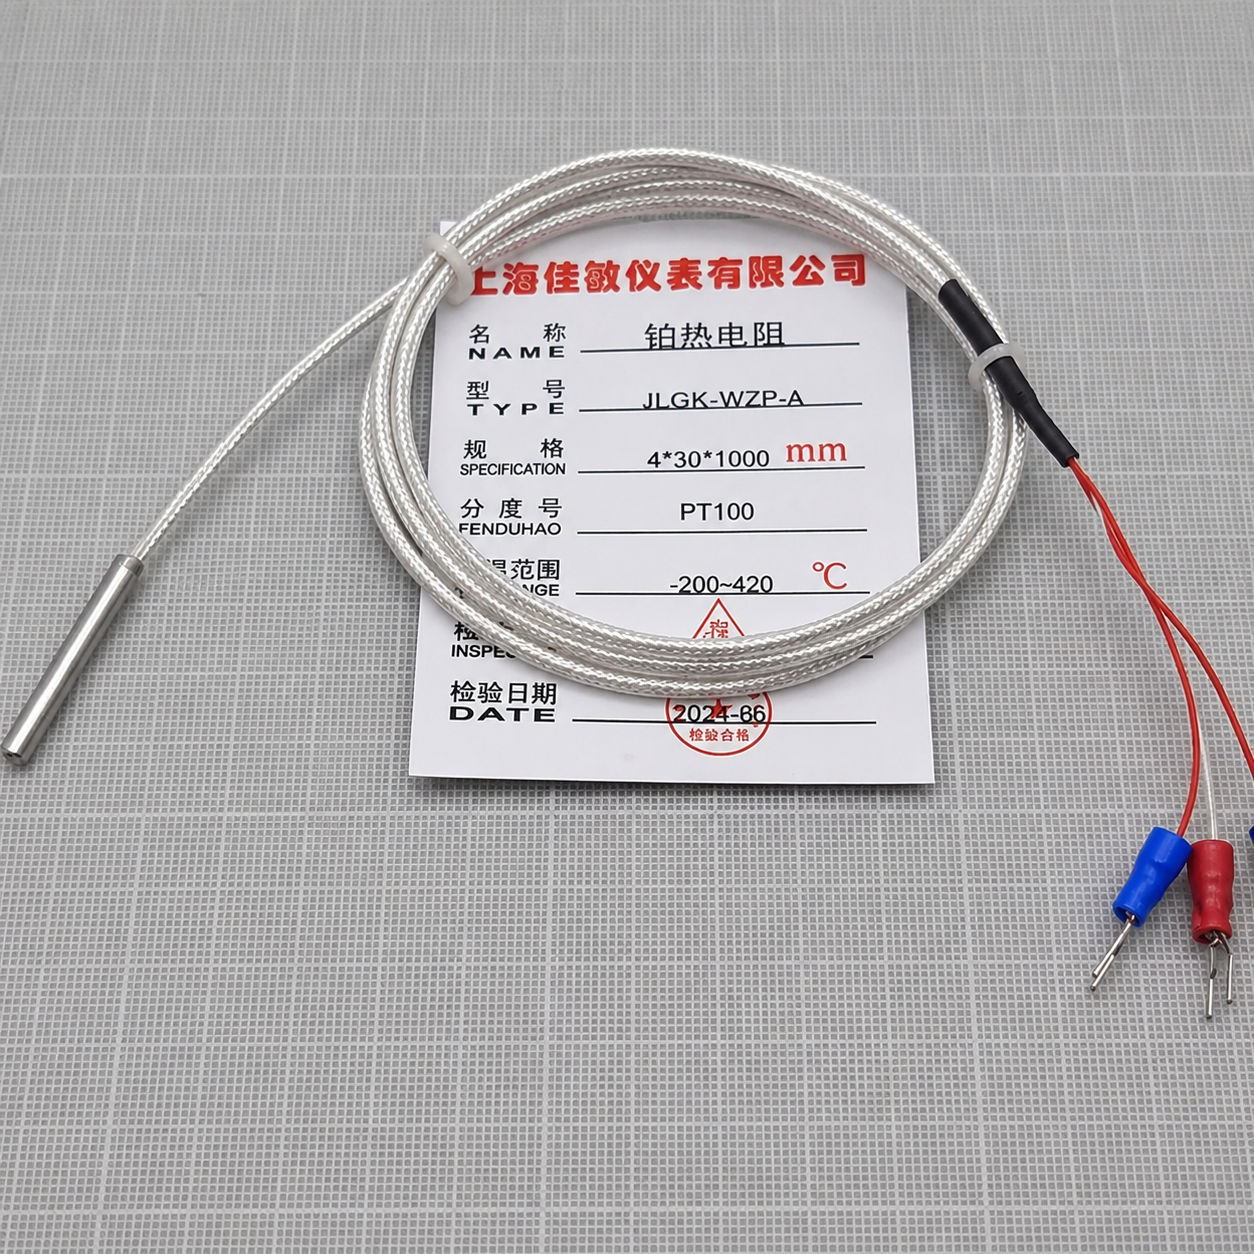
\includegraphics[width=\linewidth,height=4cm,keepaspectratio]{assets/gambar/gambar-4-04-pt100.png}
  \end{minipage}\hfill
  \begin{minipage}[c]{0.46\linewidth}
    \centering
    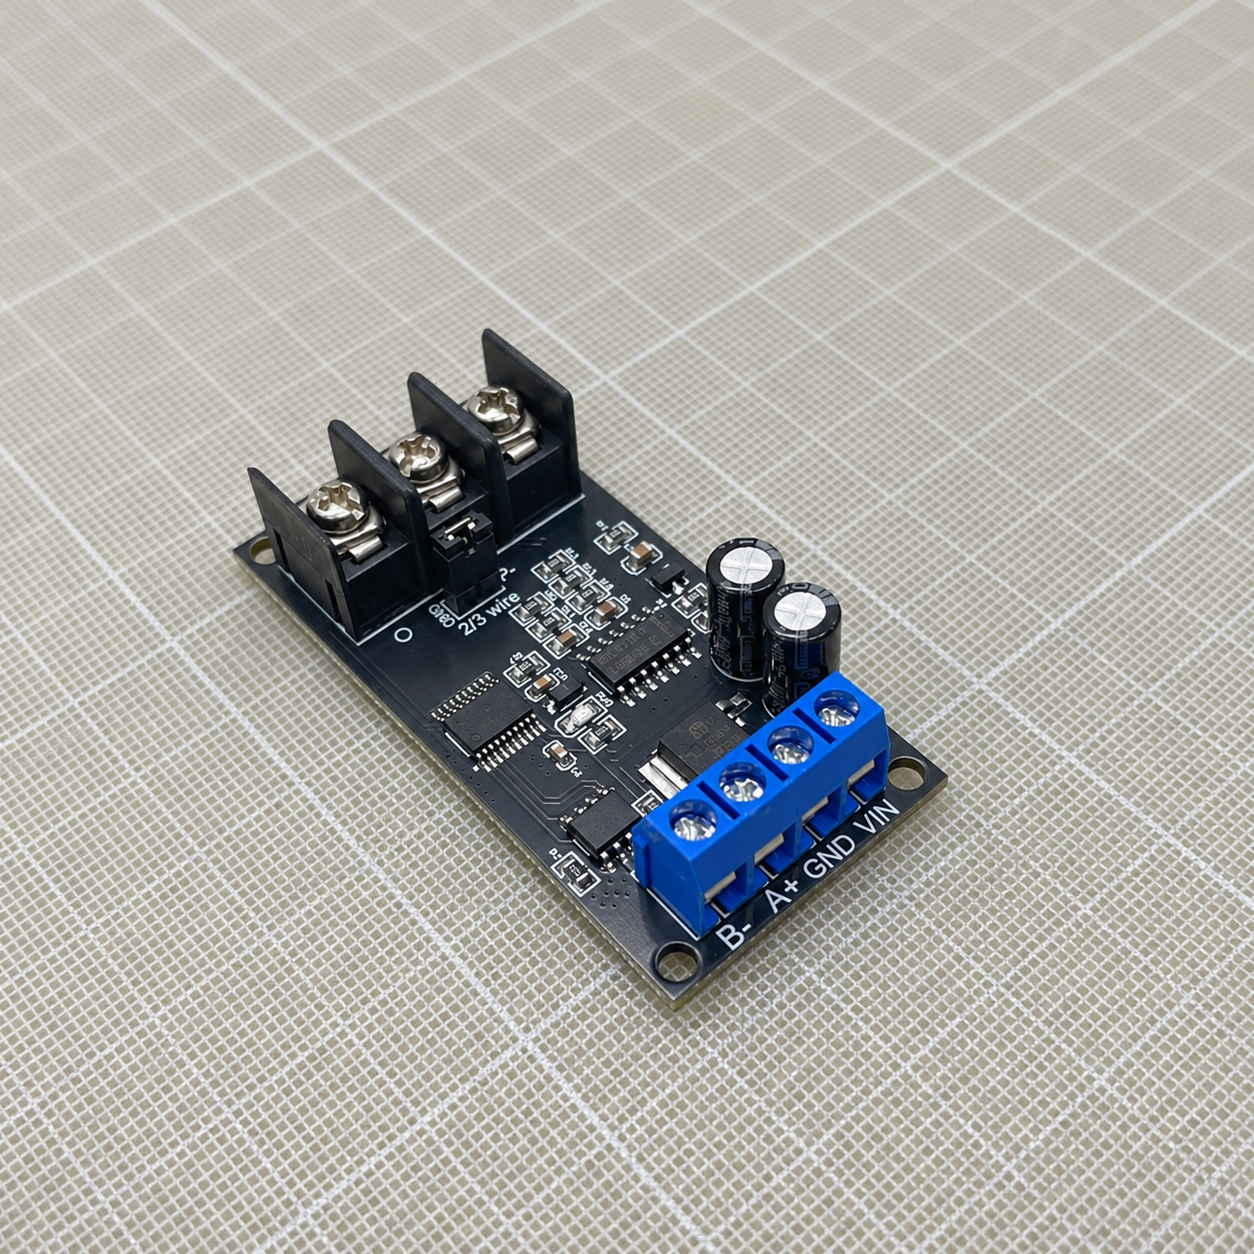
\includegraphics[width=\linewidth,height=4cm,keepaspectratio]{assets/gambar/gambar-4-04-konverter.png}
  \end{minipage}
  \caption{Sensor PT100 dan Konverter RTD--RS485}\label{fig:draft-3-4}
\end{figure}

% DOCX block 518
\Needspace{10cm}
\subsubsection{Transduser Arus untuk Pengukuran Tiga Fasa}

% DOCX block 519
Setiap transduser arus hanya mengukur arus pada satu fasa. Oleh karena itu, pengukuran arus tiga fasa menggunakan tiga transduser, masing-masing untuk fasa R, S, dan T. Dalam implementasi digunakan dua jenis transduser berdasarkan keluarannya, yaitu arus DC 4--20 mA dan tegangan DC 0--5 V. Penggunaan kedua jenis ini merupakan penyesuaian terhadap keterbatasan ketersediaan barang di pasaran. Keduanya dapat diterima oleh modul masukan analog Waveshare, dengan penyesuaian jenis masukan pada kanal masing-masing.

Transduser pada Gambar~\ref{fig:draft-3-5} merupakan jenis keluaran 4--20 mA, dengan rentang masukan arus AC 0--20 A dan catu daya 24 VDC sesuai label perangkat. Keluaran 4 mA menyatakan 0 A dan 20 mA menyatakan 20 A. Untuk jenis keluaran 0--5 V, tegangan 0 V menyatakan arus nol dan 5 V menyatakan batas atas rentang ukur pada label transduser yang digunakan.

Kanal untuk transduser 4--20 mA diatur sebagai masukan arus, sedangkan kanal untuk transduser 0--5 V diatur sebagai masukan tegangan. Aplikasi menerapkan konversi sesuai jenis sinyal: \(I_{\mathrm{fasa}}=(I_{\mathrm{out}}-4)\times I_{\mathrm{maks}}/16\) untuk keluaran 4--20 mA, dan \(I_{\mathrm{fasa}}=V_{\mathrm{out}}\times I_{\mathrm{maks}}/5\) untuk keluaran 0--5 V. Dalam hubungan tersebut, \(I_{\mathrm{out}}\) dinyatakan dalam mA, \(V_{\mathrm{out}}\) dalam volt, serta \(I_{\mathrm{maks}}\) dan \(I_{\mathrm{fasa}}\) dalam ampere. Nilai \(I_{\mathrm{maks}}\) mengikuti rentang ukur masing-masing transduser. Pemetaan kanal tetap membedakan fasa R, S, dan T, sehingga perbedaan jenis keluaran tidak mengubah parameter arus yang disajikan pada HMI.

% DOCX block 520
\GambarLaporan{assets/gambar/gambar-4-05.jpg}{Transduser Arus Satu Fasa}{fig:draft-3-5}{}

% DOCX block 521
\Needspace{12cm}
\subsubsection{Sensor Tekanan SMC ISE30A-01-D}

% DOCX block 522
Sensor tekanan SMC ISE30A-01-D digunakan untuk mengukur tekanan udara. Kode keluaran D menyediakan satu keluaran sakelar NPN dan keluaran arus analog. Pada rentang tekanan positif 0--1 MPa atau 0--10 bar, keluaran arusnya adalah 4--20 mA DC: 4 mA menyatakan 0 MPa dan 20 mA menyatakan 1 MPa. Rentang nominal sensor mencakup \(-0{,}1\) hingga 1 MPa, sehingga keluaran pada batas tekanan negatif tersebut dapat mencapai 2,4 mA \citep{smcise30a}.

Keluaran arus dihubungkan ke kanal masukan arus Waveshare untuk memperoleh nilai tekanan kontinu. Hubungan konversinya adalah \(P=(I_{\mathrm{out}}-4)/16\), dengan \(I_{\mathrm{out}}\) dalam mA dan \(P\) dalam MPa. Keluaran sakelar NPN merupakan sinyal diskret dan dibedakan dari keluaran arus yang digunakan untuk pembacaan tekanan.

% DOCX block 523
\par\nopagebreak[3]
\begin{figure}[H]
  \centering
  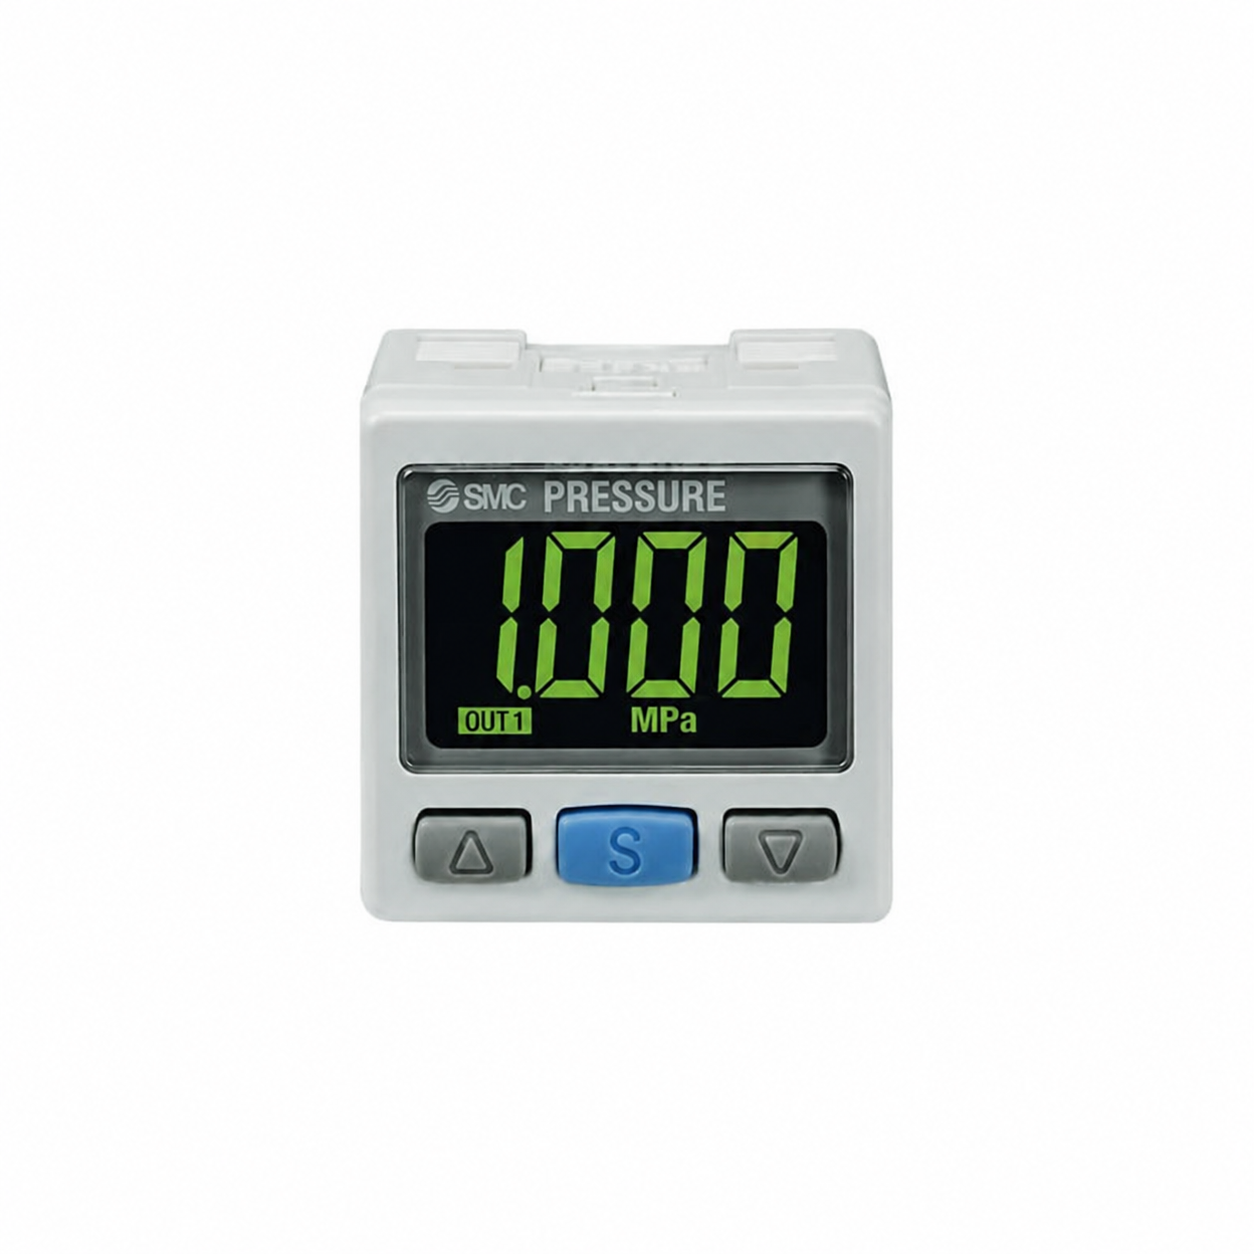
\includegraphics[trim={242bp 219bp 242bp 217bp},clip,width=.78\linewidth,height=4.8cm,keepaspectratio]{assets/gambar/gambar-4-06.png}
  \caption{Sensor Tekanan SMC ISE30A-01-D}\label{fig:draft-3-6}
\end{figure}

% DOCX block 524
\Needspace{12cm}
\subsubsection{Sensor Aliran SMC PFMB7202-06-C}

% DOCX block 525
Sensor aliran SMC PFMB7202-06-C memiliki rentang ukur nominal 20--2000 L/min. Kode keluaran C menyediakan satu keluaran sakelar NPN dan keluaran tegangan analog 1--5 VDC. Karakteristik tegangan menggunakan titik acuan 1 V pada 0 L/min dan 5 V pada 2000 L/min; pada batas ukur nominal 20 L/min, tegangannya sekitar 1,04 V \citep{smcpfmb}. Dengan demikian, titik acuan nol pada konversi dibedakan dari batas bawah rentang ukur nominal sensor.

Keluaran tegangan dihubungkan ke kanal masukan tegangan Waveshare dan dikonversi melalui \(Q=(V_{\mathrm{out}}-1)\times 500\), dengan \(V_{\mathrm{out}}\) dalam volt dan \(Q\) dalam L/min. Pada pengolahan siklus, nilai laju aliran digunakan untuk menentukan awal dan akhir siklus serta menyusun ringkasan nilai aliran.

% DOCX block 526
\par\nopagebreak[3]
\begin{figure}[H]
  \centering
  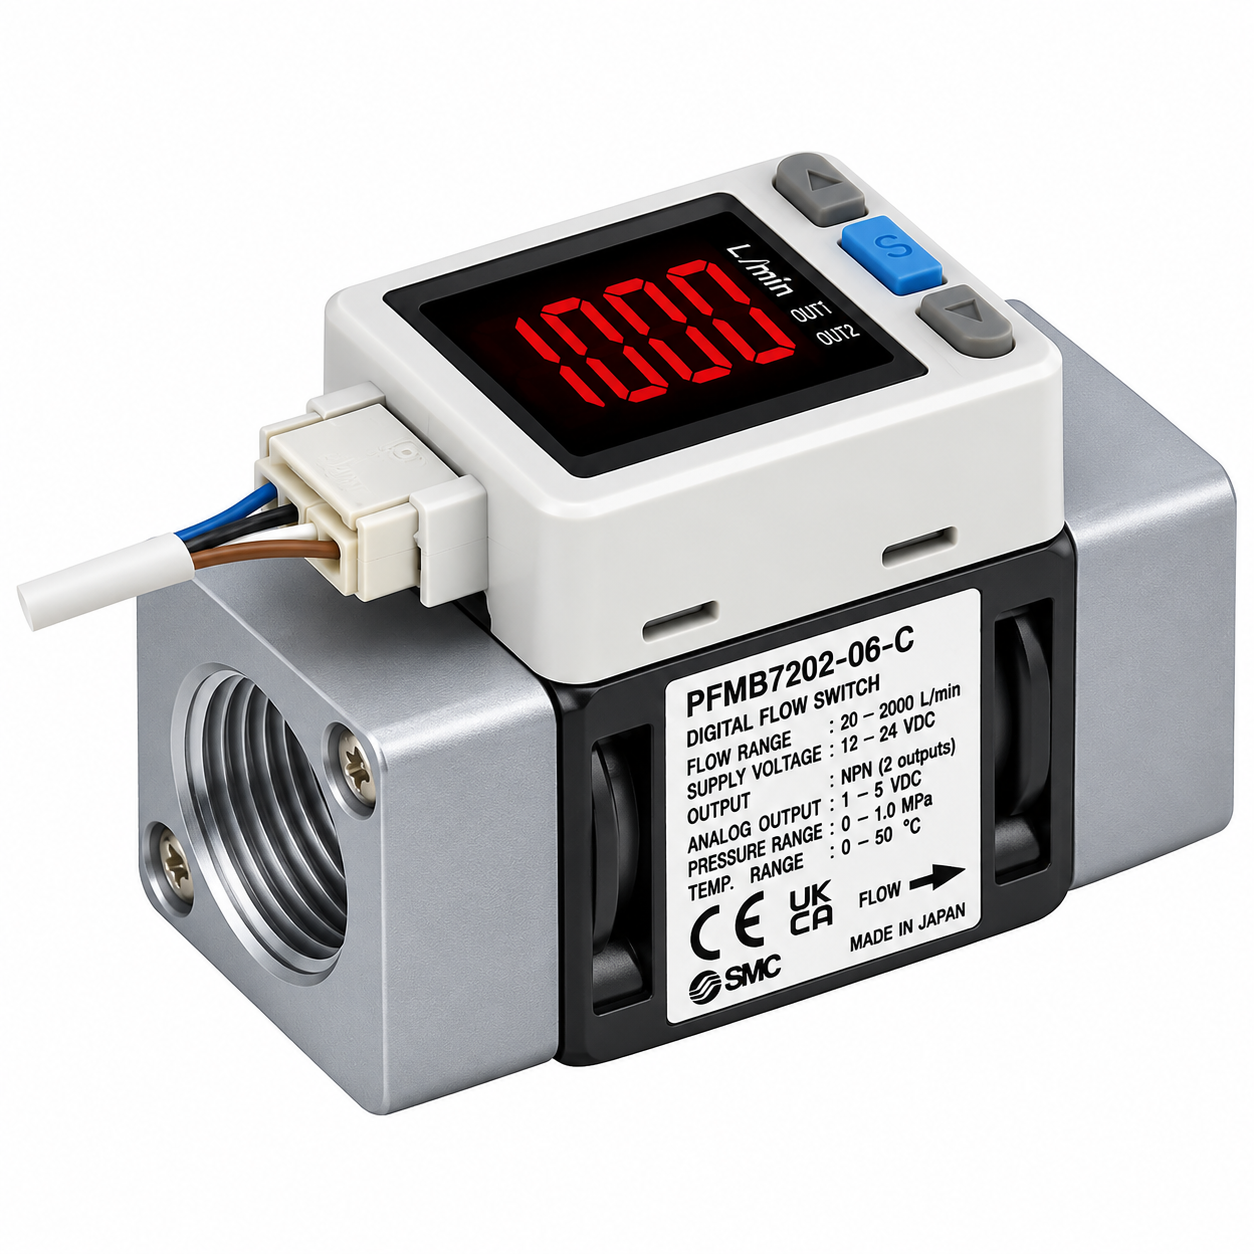
\includegraphics[trim={0bp 75bp 0bp 84bp},clip,width=.78\linewidth,height=4.8cm,keepaspectratio]{assets/gambar/gambar-4-07.png}
  \caption{Sensor Aliran SMC PFMB7202-06-C}\label{fig:draft-3-7}
\end{figure}

% DOCX block 527
\Needspace{11cm}
\subsubsection{Waveshare Modbus RTU Analog Input 8CH}

% DOCX block 528
Modul Waveshare Modbus RTU Analog Input 8CH menggunakan slave ID 2. Modul ini menerima dua jenis keluaran transduser arus, yaitu 4--20 mA DC dan 0--5 VDC, serta keluaran sensor tekanan 4--20 mA DC dan sensor aliran 1--5 VDC. Kanal untuk transduser keluaran 4--20 mA dan sensor tekanan dikonfigurasi sebagai masukan arus. Kanal untuk transduser keluaran 0--5 V dan sensor aliran dikonfigurasi sebagai masukan tegangan. Pengaturan jumper dan rentang konversi pada aplikasi disesuaikan dengan sinyal setiap perangkat agar pembacaan tetap menghasilkan satuan teknik yang sesuai. Hasil akuisisi diakses melalui Modbus RTU sehingga masukan analog dapat diolah oleh aplikasi. Konfigurasi kanal harus sesuai jenis sinyal yang dihubungkan ke modul \citep{waveshare}.

% DOCX block 529
\par\nopagebreak[3]
\begin{figure}[H]
  \centering
  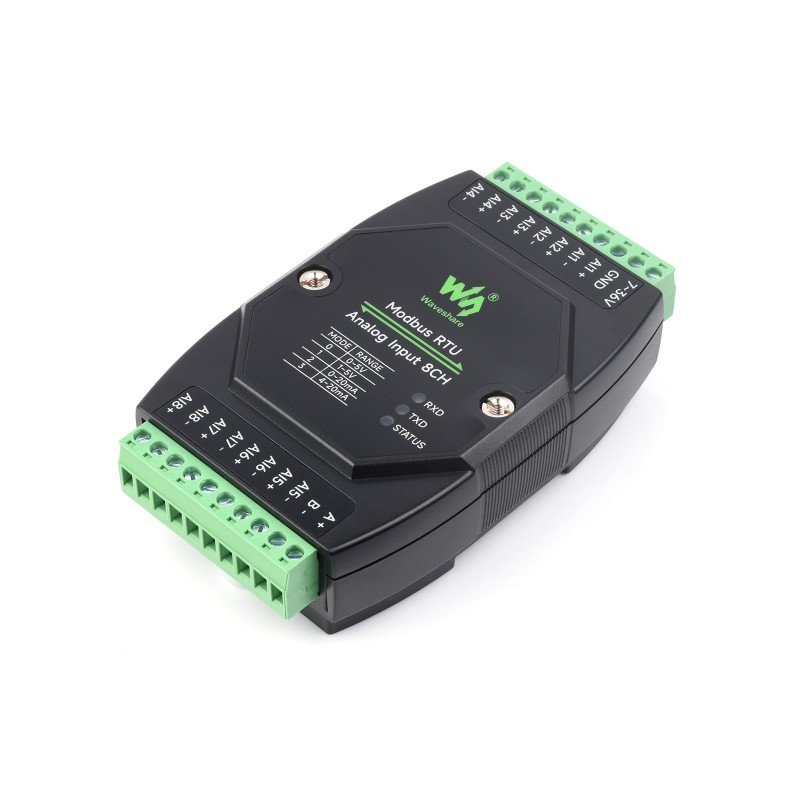
\includegraphics[trim={60bp 95bp 63bp 91bp},clip,width=.78\linewidth,height=4.8cm,keepaspectratio]{assets/gambar/gambar-4-08.jpg}
  \caption{Waveshare Modbus RTU Analog Input 8CH}\label{fig:draft-3-8}
\end{figure}

% DOCX block 530
\Needspace{6.2cm}
\subsubsection{Konverter Waveshare USB--RS485}

% DOCX block 531
Sistem menggunakan satu unit konverter Waveshare USB--RS485 untuk menghubungkan port USB Raspberry Pi dengan jalur komunikasi RS485. Konverter RTD--RS485 dan modul masukan analog Waveshare diakses melalui antarmuka yang sama menggunakan protokol Modbus RTU. Pada jalur ini, slave ID 1 digunakan untuk konverter RTD--RS485 dan slave ID 2 untuk modul Waveshare Modbus RTU Analog Input 8CH. Aplikasi menentukan slave ID dan alamat register sesuai perangkat yang akan dibaca. Konverter USB--RS485 berfungsi sebagai penghubung komunikasi, sedangkan modul Waveshare Modbus RTU Analog Input 8CH berfungsi membaca sinyal arus dan tegangan dari sensor.

% DOCX block 532
\GambarLaporan{assets/gambar/gambar-4-09.jpg}{Konverter Waveshare USB--RS485}{fig:draft-3-9}{}

% DOCX block 533
\Needspace{8cm}
\subsubsection{Catu Daya 5 VDC dan 24 VDC}

% DOCX block 534
Catu daya 5 VDC disediakan khusus untuk Raspberry Pi. Catu daya 24 VDC digunakan untuk perangkat pengukuran, konverter, dan buzzer sesuai susunan sistem. Pembagian catu daya diperhatikan dalam pemasangan agar kebutuhan setiap perangkat terpenuhi.

% DOCX block 535
\par\nopagebreak[3]
\begin{figure}[H]
  \centering
  \begin{minipage}[c]{0.46\linewidth}
    \centering
    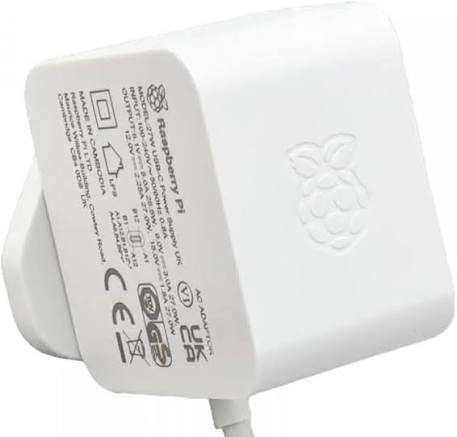
\includegraphics[width=\linewidth,height=4cm,keepaspectratio]{assets/gambar/gambar-4-10-5v.jpg}
  \end{minipage}\hfill
  \begin{minipage}[c]{0.46\linewidth}
    \centering
    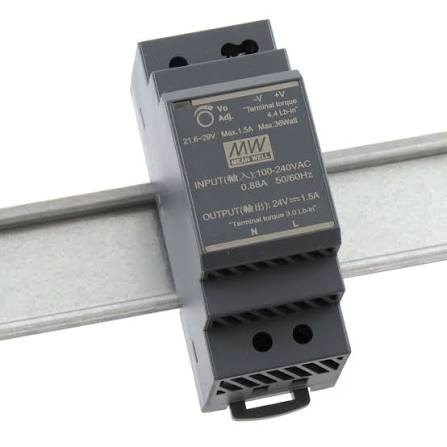
\includegraphics[width=\linewidth,height=4cm,keepaspectratio]{assets/gambar/gambar-4-10-24v.jpg}
  \end{minipage}
  \caption{Catu Daya 5 VDC dan 24 VDC}\label{fig:draft-3-10}
\end{figure}

% DOCX blocks 536--538: perangkat alarm dipisahkan sesuai fungsi.
\Needspace{6.2cm}
\subsubsection{Pembaca RFID}

Pembaca RFID digunakan untuk membaca identitas kartu teknisi sebagai masukan dalam penanganan peringatan. Identitas kartu dikirim melalui antarmuka USB ke Raspberry Pi, kemudian diperiksa oleh aplikasi sebelum penanganan buzzer diproses. Aktivitas penanganan dicatat bersama informasi alarm agar dapat ditelusuri.

\GambarLaporan{assets/gambar/gambar-4-11-rfid.jpg}{Pembaca RFID}{fig:draft-3-11}{}

\Needspace{6.2cm}
\subsubsection{Modul Relay}

Modul relay berfungsi sebagai sakelar untuk menyambungkan atau memutus suplai 24 VDC ke buzzer. Raspberry Pi mengendalikan modul melalui GPIO, sedangkan kontak relay mengatur jalur catu daya buzzer. Polaritas sinyal kendali disesuaikan dengan modul yang digunakan.

\GambarLaporan{assets/gambar/gambar-relay.jpg}{Modul Relay}{fig:modul-relay}{}

\Needspace{6.8cm}
\subsubsection{Buzzer 24 VDC}

Buzzer 24 VDC digunakan sebagai keluaran peringatan suara ketika alarm aktif. Suplai daya buzzer dikendalikan melalui kontak relay sesuai perintah aplikasi. Fungsi ini melengkapi peringatan visual pada HMI agar kondisi alarm dapat diketahui oleh pengguna di area mesin.

\begingroup
\setlength{\BatasTinggiGambar}{3.3cm}
\GambarLaporan{assets/gambar/gambar-4-11-buzzer.jpg}{Buzzer 24 VDC}{fig:buzzer-24v}{}
\endgroup

Dalam sistem alarm, aplikasi mengaktifkan buzzer melalui relay ketika alarm terdeteksi. Pembaca RFID menyediakan identitas teknisi untuk penanganan peringatan. Ketiganya berfungsi sebagai masukan identitas, pengendali jalur daya, dan keluaran suara.

% DOCX block 539
\setlength{\TinggiRuangGambar}{3.2cm}
\setlength{\BatasTinggiGambar}{0.58\textheight}
\captionsetup[figure]{skip=12pt}
\subsection{Penyesuaian Konfigurasi Mesin Cutting}

% DOCX block 540
Setiap mesin cutting menggunakan alur yang sama: membaca perangkat melalui RS485/Modbus RTU, mengolah data pada Raspberry Pi, menampilkannya pada HMI, dan mengirimkannya ke server. Pengaturan perangkat dan pengolahan data disesuaikan untuk setiap mesin.

% DOCX block 541
Pengaturan aplikasi meliputi identitas mesin, alamat perangkat, kanal sensor, port komunikasi, dan batas parameter. Pada konfigurasi yang memakai pengolahan siklus aliran udara, aplikasi juga menampilkan nilai tertinggi dan terendah positif setiap siklus.

% DOCX block 542
Tampilan yang sama memudahkan pengguna membaca informasi pada kedua mesin. Pengaturan setiap mesin tetap terpisah agar nilai yang ditampilkan sesuai dengan sensor dan kanal yang terpasang.

% DOCX block 543
\subsection{Pengembangan Perangkat atau Modul Pendukung}

% DOCX block 544
Selain membaca sensor, aplikasi menyediakan alarm, pemeriksaan kartu RFID, pengaturan sensor, ekspor data, dan pengiriman riwayat ke server. Pengaturan jarak jauh melalui MQTT dapat digunakan jika layanannya diaktifkan.

% DOCX block 545
\subsubsection{Deteksi alarm dan autentikasi RFID}

% DOCX block 546
AlarmService membandingkan pembacaan baru dengan batas minimum dan maksimum. Alarm parameter dipicu setelah tiga sampel berturut-turut berada di luar batas. Pembacaan normal mereset penghitung, sedangkan nilai yang tidak tersedia dilewati dalam evaluasi. Saat alarm aktif, HMI menampilkan perubahan indikator dan peringatan serta mengendalikan buzzer 24 VDC melalui relay.

% DOCX block 547
Pembaca RFID menggunakan antarmuka USB HID untuk mengirimkan identitas kartu. Aplikasi mencocokkan identitas tersebut dengan daftar teknisi pada SQLite sebelum memproses penanganan buzzer. Aktivitas penanganan dicatat bersama riwayat alarm agar dapat ditelusuri. Raspberry Pi mengendalikan relay melalui GPIO dengan polaritas pemicu sesuai modul yang digunakan. Kontak relay menghubungkan atau memutus suplai 24 VDC ke buzzer.

% DOCX block 548
\subsubsection{Pengaturan modul dan sensor jarak jauh}

% DOCX block 549
Pengaturan jarak jauh menggunakan perintah MQTT untuk membaca konfigurasi modul, mengubah batas alarm, serta mengatur alamat perangkat dan mode kanal. Perintah masuk ke antrean pada proses pengelola port serial agar tidak dijalankan bersamaan dengan pembacaan sensor. Beberapa perubahan disertai pemeriksaan nilai, pembacaan ulang, dan konfirmasi hasil ke dashboard. Fitur ini dapat digunakan jika layanannya diaktifkan.

% DOCX block 550
Pengaturan melalui perangkat lunak harus sesuai dengan posisi jumper dan karakteristik masukan perangkat. Rentang konversi serta offset ditetapkan berdasarkan sensor yang terpasang. Oleh karena itu, perubahan konfigurasi perlu disertai pemeriksaan kesesuaian kanal dan sinyal agar nilai yang ditampilkan tetap mewakili besaran yang diukur.

% Pembahasan panel berdasarkan program yang diberikan dan konfirmasi pengguna.
\subsection{Perancangan dan Implementasi Sistem Monitoring Panel Listrik}
\label{sec:monitoring-panel}

Proyek monitoring panel listrik merupakan lingkup pekerjaan Muhammad Fadhil Abdillah. Sistem menghimpun parameter kelistrikan serta kondisi suhu dan kelembaban panel, mengevaluasi peringatan pada sisi perangkat, dan menyajikan informasi melalui dashboard server. Konfigurasi yang telah berjalan di area Power Room menggunakan satu Raspberry Pi untuk melayani empat panel yang berdekatan, dengan modul MAX3485 sebagai antarmuka RS485. Rancangan pengembangannya menempatkan satu unit monitoring pada setiap blok panel.

Pembahasan panel meliputi aplikasi pada Raspberry Pi, dashboard server, dan penerapan satu node untuk empat panel di Power Room. Konfigurasi awal program digunakan untuk menjelaskan pengalamatan dan alur pembacaan. Diagram beberapa node menggambarkan rancangan perluasan monitoring untuk blok panel lain.

\subsubsection{Kebutuhan dan pembagian fungsi sistem}

Panel listrik memerlukan pemantauan parameter sumber dan beban, konsumsi energi, serta kondisi lingkungan di dalam panel. Pembacaan setiap panel perlu dibedakan berdasarkan identitasnya agar perubahan parameter dan alarm dapat ditelusuri. Pada satu blok, Raspberry Pi berfungsi sebagai pengumpul data sekaligus pelaksana evaluasi alarm, sedangkan dashboard menyediakan pemantauan beberapa panel, histori, analisis, dan pengaturan.

Sistem panel membaca data kelistrikan dari Schneider Electric PM2120 serta suhu dan kelembaban dari THM30MD. Nama PM2120 mengikuti perangkat yang dibaca program; dokumentasi resmi menempatkannya dalam seri EasyLogic PM2100 \citep{schneiderpm2100}. Kedua perangkat mengirim data digital melalui Modbus RTU. Berbeda dari sistem cutting yang membaca sinyal transduser melalui modul analog, sistem panel menggunakan modul MAX3485 yang terhubung ke UART Raspberry Pi.

\subsubsection{Arsitektur satu blok satu node}

Gambar~\ref{fig:panel-arsitektur} menunjukkan pola hubungan perangkat pada sistem panel. Setiap node mewakili satu Raspberry Pi beserta antarmuka RS485 dan pembaca RFID Wiegand dengan buzzer serta LED terintegrasi. Perangkat ukur beberapa panel dalam blok diakses secara bergantian melalui alamat Modbus. Pada konfigurasi yang berjalan, satu node tersebut melayani empat panel di Power Room. Jumlah node dan panel pada diagram merupakan pola perluasan, bukan jumlah pemasangan aktual.

% Diagram fungsional berdasarkan diagram pengguna dan program panel.
% Node pertama terpasang; node berikutnya merupakan rancangan pengembangan.
\begin{figure}[tbp]
\centering
\begin{tikzpicture}[
 font=\rmfamily\fontsize{8}{9.5}\selectfont,
 box/.style={draw=blue!45!black,rounded corners=2pt,align=center,
 fill=blue!3,inner sep=4pt,text width=2.55cm},
 link/.style={->,thick,draw=blue!45!black}]
\node[box,fill=blue!65!black,text=white] at (-3.15,0)
 {\textbf{Node 1}\\Power Room\\4 panel terpasang};
\node[box,dashed,fill=gray!8] at (0,0)
 {\textbf{Node 2}\\Rancangan blok berikutnya};
\node[box,dashed,fill=gray!8] at (3.15,0)
 {\textbf{Node N}\\Rancangan perluasan};
\foreach \x/\name in {-3.15/a,0/b,3.15/c}{
 \node[box] (meter\name) at (\x,-1.8)
  {\textbf{Perangkat tiap panel}\\PM2120 dan THM30MD};
 \node[box] (pi\name) at (\x,-3.6)
  {\textbf{Raspberry Pi}\\XY-017 (MAX3485)\\Akuisisi dan alarm};
 \draw[link] (meter\name) -- node[right,font=\rmfamily\fontsize{7}{8}\selectfont]
  {RS485} (pi\name);
 \node[box] (alarm\name) at (\x,-5.25)
  {RFID Wiegand D0/D1\\Buzzer/LED bawaan\\Catu reader 12 V};
 \draw[<->,thick,blue!45!black] (pi\name) -- (alarm\name);
 \draw[thick,blue!45!black] (pi\name.east) -- (\x+1.53,-3.6) -- (\x+1.53,-6.3);
}
\draw[thick,blue!45!black] (-1.62,-6.3) -- (4.68,-6.3);
\node[fill=white,inner sep=2pt] at (0,-6.3) {Ethernet melalui switch};
\node[box,text width=8.8cm] (broker) at (0,-7.5)
 {\textbf{Broker MQTT}\\Menyalurkan telemetri, status node, dan perintah};
\draw[link] (0,-6.43) -- (broker);
\node[box,text width=8.8cm] (server) at (0,-8.95)
 {\textbf{Dashboard server panel}\\Django, basis data, histori, alarm, statistik, dan ekspor};
\draw[<->,thick,blue!45!black] (broker) -- (server);
\end{tikzpicture}
\caption{Arsitektur monitoring panel dan pengembangan per blok}
\label{fig:panel-arsitektur}
\end{figure}


Dalam rancangan jaringan, node terhubung melalui Ethernet ke switch dan server dashboard. Data pengukuran dan perintah dikirim melalui MQTT. Switch menghubungkan perangkat pada jaringan, sedangkan broker MQTT menyalurkan pesan sesuai topiknya. Alamat broker diatur melalui konfigurasi program. Akun dan alamat internal tidak dicantumkan untuk menjaga kerahasiaan jaringan perusahaan.

Program memakai tiga jenis identitas. \textit{Device ID} menunjukkan node Raspberry Pi, \textit{panel ID} menunjukkan panel, dan slave ID memilih perangkat Modbus. Pada basis data server, setiap panel ID harus berbeda di seluruh sistem. Nomor panel pada ilustrasi beberapa blok tidak dapat digunakan berulang tanpa penyesuaian. Penambahan panel juga harus memperhatikan waktu pembacaan, keunikan alamat pada bus, dan kapasitas perangkat.

\subsection{Komponen Perangkat Keras Monitoring Panel}
\label{sec:komponen-panel}

Perangkat monitoring panel dibagi menjadi unit pengolah, perangkat ukur, antarmuka komunikasi, dan perangkat peringatan. Satu unit pengolah melayani empat panel di Power Room. Hubungan komponen mengikuti arsitektur pada Gambar~\ref{fig:panel-arsitektur}, sedangkan fungsi masing-masing dijelaskan sebagai berikut.

\Needspace{6cm}
\subsubsection{Raspberry Pi}

Raspberry Pi menjadi komputer utama pada node monitoring panel. Model yang digunakan pada kedua proyek dijelaskan pada Subbab~\ref{sec:raspberry-pi}. Pada sistem panel, Raspberry Pi membaca meter dan sensor, membandingkan hasilnya dengan batas alarm, menerima identitas kartu RFID melalui D0 dan D1, serta mengendalikan peringatan buzzer dan LED pada reader. Data dikirim melalui MQTT ke dashboard server. Satu Raspberry Pi menangani empat panel yang berdekatan dalam satu blok.

% Dokumentasi yang diperlukan: Foto unit lengkap yang memperlihatkan Raspberry Pi, modul antarmuka, dan perangkat pendukung.
\GambarLaporan{assets/gambar/panel-01-unit.png}{Unit monitoring panel berbasis Raspberry Pi}{fig:panel-unit}{}

\Needspace{6cm}
\subsubsection{Meter Schneider Electric PM2120}

PM2120 menyediakan data kelistrikan panel, meliputi tegangan, arus, frekuensi, daya aktif, faktor daya, dan energi. Aplikasi membaca data tersebut dari register meter melalui Modbus RTU. Dokumentasi pabrikan menempatkan PM2120 dalam seri EasyLogic PM2100 \citep{schneiderpm2100}. Pada program, identitas panel dipasangkan dengan slave ID meter agar hasil pembacaan dapat ditampilkan untuk panel yang tepat.

% Dokumentasi yang diperlukan: Foto meter pada panel, dengan model dan tampilan pembacaan terbaca.
\GambarLaporan{assets/gambar/panel-02-pm2120.png}{Meter Schneider Electric PM2120 pada panel listrik}{fig:panel-pm2120}{}

\Needspace{6cm}
\subsubsection{Sensor Suhu dan Kelembaban THM30MD}

THM30MD digunakan untuk memantau suhu dan kelembaban di dalam panel. Data lingkungan ini melengkapi pengukuran kelistrikan dari PM2120. Aplikasi membaca kedua nilai melalui Modbus RTU, kemudian menampilkannya pada dashboard dan membandingkannya dengan batas alarm.

Keluaran yang dibaca program berupa data digital suhu dan kelembaban. Program membaca empat register mulai alamat heksadesimal 02, lalu menggabungkan setiap dua register menjadi bilangan pecahan 32 bit. Bentuk penyimpanan data tersebut berbeda dari rentang fisik dan akurasi sensor; nilai spesifikasi perangkat mengikuti label unit dan manual pabrikan.

% Dokumentasi yang diperlukan: Foto sensor dan posisi pemasangannya di panel.
\GambarLaporan{assets/gambar/panel-03-thm30md.png}{Sensor suhu dan kelembaban THM30MD pada panel}{fig:panel-thm30md}{}

\Needspace{6cm}
\subsubsection{Modul XY-017 Berbasis MAX3485}

Modul RS485 yang digunakan adalah XY-017 berbasis IC MAX3485. Modul ini menghubungkan UART Raspberry Pi dengan bus RS485 untuk pertukaran data bersama PM2120 dan THM30MD. IC MAX3485 menjalankan fungsi pengirim dan penerima sinyal RS485 \citep{max3485}. UART menyediakan data serial pada Raspberry Pi, sedangkan format permintaan dan balasan perangkat mengikuti Modbus RTU. Identitas perangkat dipilih melalui slave ID. Perangkat keras ini berbeda dari adapter USB--RS485 yang digunakan pada monitoring cutting.

% Dokumentasi yang diperlukan: Foto modul XY-017 berbasis MAX3485 yang digunakan pada unit monitoring panel; tulisan tipe modul dibuat terbaca.
\GambarLaporan{assets/gambar/panel-15-max3485.png}{Modul XY-017 berbasis MAX3485 pada monitoring panel}{fig:panel-max3485}{}

\Needspace{4cm}
\subsubsection{Pembaca RFID Wiegand dengan Buzzer dan LED Terintegrasi}

Pembaca RFID panel mengirim identitas kartu melalui jalur D0 dan D1 dengan antarmuka Wiegand. Jenis ini berbeda dari pembaca USB RFID pada mesin cutting. Program menyusun pulsa dari D0 dan D1 menjadi identitas kartu, kemudian memeriksanya terhadap daftar kartu pada node.

Buzzer dan LED sudah terintegrasi di dalam RFID reader. Reader memperoleh catu daya dari jalur 12 V pada rangkaian daya PCB. Satu perangkat digunakan bersama untuk panel-panel yang dilayani oleh node. Buzzer menyediakan peringatan suara, sedangkan LED menyediakan tanda visual. Dengan susunan ini, pembacaan kartu dan peringatan berada pada satu perangkat fisik.

Program menentukan peringatan berdasarkan status alarm panel. Setelah penanganan kartu, buzzer dapat diredam sesuai alur aplikasi. Status mute tidak mengubah hasil pengukuran atau menyatakan bahwa penyebab alarm sudah kembali normal. Program menggunakan indikasi hijau untuk kondisi normal dan merah untuk alarm; setelah penanganan, indikasi merah berkedip lambat selama alarm masih ada. Urutan penanganan kartu dibahas pada bagian program panel.

% Dokumentasi yang diperlukan: Foto RFID reader panel dengan keluaran Wiegand D0/D1 serta buzzer dan LED bawaan; tampilkan perangkat utuh dan identitasnya bila tersedia.
\GambarLaporan{assets/gambar/panel-05-rfid-alarm.png}{Pembaca RFID Wiegand dengan buzzer dan LED terintegrasi}{fig:panel-rfid-alarm}{}

\Needspace{5cm}
\subsubsection{Rangkaian Catu Daya}

Sumber daya monitoring panel menggunakan power supply 24 V. Tegangan ini diturunkan menjadi 12 V melalui modul step-down XL4015 untuk memasok RFID reader. Susunan ini mengikuti skematik pada Gambar~\ref{fig:panel-skematik}.

Jalur 12 V memasok RFID reader beserta buzzer dan LED yang terintegrasi di dalamnya. Jalur daya ini dibedakan dari D0 dan D1 yang mengirim identitas kartu. Skematik juga mencantumkan sekring dan kapasitor pada bagian catu daya. Dokumentasi bagian daya PCB ditunjukkan pada Gambar~\ref{fig:panel-adaptor-12v}.

% Dokumentasi yang diperlukan: Foto bagian daya PCB monitoring panel yang memperlihatkan modul XL4015, regulator, dan konektor catu; dapat memakai gambar detail bagian POWER dari skematik asli.
\GambarLaporan{assets/gambar/panel-16-catu-daya.png}{Rangkaian catu daya PCB monitoring panel}{fig:panel-adaptor-12v}{}

\subsubsection{Skematik dan Layout PCB Antarmuka Panel}
\label{sec:skematik-pcb-panel}

Rancangan rangkaian antarmuka monitoring panel ditunjukkan pada Gambar~\ref{fig:panel-skematik}. Skematik membagi rangkaian menjadi bagian catu daya, kendali RFID, dan komunikasi RS485. Bagian catu daya menurunkan tegangan 24 V menjadi 12 V melalui modul XL4015 untuk RFID reader. Bagian RFID memuat konektor reader, jalur D0 dan D1, jaringan resistor, serta transistor Q1 dan Q2 berlabel BC547 pada jalur kendali buzzer dan LED. Buzzer dan LED tetap berada di dalam RFID reader, sedangkan rangkaian pada PCB menyediakan jalur antarmukanya.

Bagian RS485 pada skematik memuat modul XY-017 berbasis MAX3485 dan konektor menuju perangkat lapangan. Konektor serta nama sinyal digunakan untuk menelusuri hubungan antarbagian rangkaian. Penempatan fisik komponen dan jalur sambungannya ditunjukkan pada layout PCB dalam Gambar~\ref{fig:panel-pcb}. Layout memperlihatkan pad komponen, lubang pemasangan, konektor, serta jalur yang menghubungkan bagian daya, RFID, dan komunikasi pada satu papan.

% Gambar pengguna terlihat pada percakapan; berkas PNG/JPG asli perlu ditempatkan pada path berikut sebelum penyisipan gambar aktual.
\GambarLaporan{assets/gambar/panel-17-skematik.png}{Skematik rangkaian antarmuka monitoring panel}{fig:panel-skematik}{}

\GambarLaporan{assets/gambar/panel-18-pcb.png}{Layout PCB rangkaian antarmuka monitoring panel}{fig:panel-pcb}{}

\subsubsection{Jaringan Ethernet dan Switch}

Dalam rancangan jaringan, Ethernet menghubungkan node dengan layanan server melalui switch. Switch meneruskan komunikasi jaringan antarperangkat. Pesan pengukuran dan perintah aplikasi disalurkan oleh broker MQTT, sehingga fungsi switch dibedakan dari layanan pesan. Susunan beberapa node pada diagram menjadi rancangan pengembangan untuk blok panel lain.

\subsubsection{Komputer Server}

Komputer server menjalankan dashboard monitoring panel berbasis Django dan layanan penerima MQTT. Server mengelola data pengukuran, riwayat, alarm, statistik, ekspor, serta pengaturan panel. Pengguna mengakses informasi melalui halaman web. Pembagian ini menempatkan pembacaan perangkat dan peringatan pada Raspberry Pi, sedangkan penyajian serta pengelolaan data terpusat berada pada server.

\subsection{Program dan Komunikasi Sistem Monitoring Panel}
\label{sec:program-panel}

Program panel menghubungkan pembacaan perangkat, pemeriksaan alarm, pengiriman data, dan dashboard. Pembahasan berikut menjelaskan parameter yang diolah, pemetaan register, urutan pembacaan, serta penanganan peringatan berdasarkan komponen pada Subbab~\ref{sec:komponen-panel}.

\subsubsection{Parameter dan keluaran perangkat pengukuran}

Tabel~\ref{tab:panel-parameter} merangkum data yang dibaca atau diolah program, bukan seluruh kemampuan meter. Tegangan dan arus menunjukkan kondisi kelistrikan, daya aktif menyatakan laju penggunaan energi, sedangkan energi aktif bersifat akumulatif. Suhu dan kelembaban menunjukkan kondisi lingkungan panel.

\Needspace{7cm}
\begin{longtblr}[caption={Parameter pada program monitoring panel},label={tab:panel-parameter}]{colspec={X[1.5,l] X[1.5,l] X[2,l]},rowhead=1,cells={valign=t},row{1}={font=\bfseries,bg=gray!15},colsep=3pt,rowsep=1.5pt}
Kelompok & Besaran dan satuan & Sumber atau pengolahan \\
Tegangan & R--S, S--T, T--R dan R--N, S--N, T--N; V & Register PM2120, disertai nilai rata-rata \\
Arus & R, S, T, netral, dan rata-rata; A & Register PM2120 \\
Daya aktif & Per fasa dan total; kW & Register PM2120 \\
Faktor daya & Per fasa; tanpa satuan & Nilai register diinterpretasikan oleh aplikasi \\
Frekuensi & Hz & Register PM2120 \\
Energi aktif & Akumulasi energi; kWh & Bilangan 64 bit dalam program, dikonversi dari Wh \\
Lingkungan & Suhu; $^{\circ}$C dan kelembaban; \% & Register THM30MD \\
Ketidakseimbangan & Penyimpangan arus dan tegangan; \% & Dihitung terhadap nilai rata-rata pada program \\
\end{longtblr}

\subsubsection{Komunikasi melalui MAX3485 dan pemetaan register}

Komunikasi perangkat menggunakan UART Raspberry Pi, modul MAX3485, dan bus RS485. Aplikasi mengirim permintaan Modbus RTU secara bergantian kepada PM2120 dan THM30MD berdasarkan alamat perangkat. Bagian ini menjelaskan pengaturan komunikasi dan pemetaan register yang dibaca program.

Raspberry Pi meminta data perangkat melalui modul \texttt{modbus\_reader.py}. Pengaturan bawaan komunikasi serial adalah 19200 baud, delapan bit data, tanpa paritas, dan satu stop bit. Program menunggu balasan paling lama 0,35 detik dan memberi jeda 0,05 detik antarpembacaan. Port utama adalah \texttt{/dev/ttyAMA0}; program juga mencari beberapa port alternatif. Pengaturan ini harus sesuai dengan perangkat pada bus.

Program meminta sejumlah data dari alamat perangkat tertentu, lalu memeriksa balasannya sebelum mengolah nilai pengukuran. Permintaan menggunakan fungsi Modbus 03 untuk membaca holding register, yaitu kelompok register yang dituju. Pesan memuat slave ID, alamat awal, jumlah register, dan kode pemeriksaan CRC16. Program memeriksa panjang balasan, alamat perangkat, kode fungsi, dan CRC. Data pecahan disusun dengan urutan byte dan word big-endian sesuai kode program. Tabel~\ref{tab:panel-register} menunjukkan pemetaan alamat yang digunakan pada program panel.

\Needspace{7cm}
\begin{longtblr}[caption={Pemetaan awal register dalam program panel},label={tab:panel-register}]{colspec={X[2,l] Q[0.8,l] Q[0.8,l] X[1.4,l]},rowhead=1,cells={valign=t},row{1}={font=\bfseries,bg=gray!15},colsep=3pt}
Blok pembacaan & Alamat awal & Jumlah register & Representasi pada program \\
Arus PM2120 & 2999 & 12 & Pecahan 32 bit \\
Tegangan antar-fasa & 3019 & 8 & Pecahan 32 bit \\
Tegangan fasa--netral & 3027 & 6 & Pecahan 32 bit \\
Rata-rata tegangan fasa--netral & 3035 & 2 & Pecahan 32 bit \\
Daya aktif & 3053 & 8 & Pecahan 32 bit \\
Faktor daya & 3077 & 8 & Pecahan 32 bit \\
Frekuensi & 3109 & 2 & Pecahan 32 bit \\
Energi aktif & 3203 & 4 & Bilangan bulat 64 bit, dibagi 1000 \\
Suhu dan kelembaban THM30MD & 2 & 4 & Dua nilai pecahan 32 bit \\
\end{longtblr}

Alamat PM2120 pada tabel mengikuti offset $-1$ dalam kode. Konfigurasi awal node memuat satu panel dengan PM2120 pada slave ID 1 dan THM30MD pada slave ID 2. Konfigurasi server memuat empat panel dengan pasangan alamat 1/2, 3/4, 5/6, dan 7/8. Nilai tersebut menjelaskan susunan konfigurasi program. Penerapan di Power Room menggunakan satu Raspberry Pi untuk melayani empat panel, dengan identitas panel dan alamat Modbus sebagai pengenal sumber data.

% Dokumentasi yang diperlukan: Foto atau diagram pengawatan aktual UART Raspberry Pi, modul MAX3485, dan bus RS485 menuju perangkat panel.
\GambarLaporan{assets/gambar/panel-04-uart-rs485.png}{Pengawatan modul MAX3485 pada node monitoring panel}{fig:panel-uart}{}

\subsubsection{Siklus pembacaan dan penyimpanan pengaturan}

Saat dijalankan, aplikasi menyiapkan pembacaan Modbus, pengendali alarm, pembaca Wiegand, pemeriksaan batas parameter, dan koneksi MQTT. Aplikasi membaca panel aktif satu per satu. Hasilnya dilengkapi identitas node dan panel, nilai hasil perhitungan, serta ringkasan alarm sebelum dikirim. Setelah seluruh panel selesai dibaca, aplikasi menentukan keluaran buzzer dan LED berdasarkan alarm pada node tersebut.

Interval bawaan untuk membaca seluruh panel adalah 300 detik. Setelah pembacaan selesai, program menghitung waktu tunggu dengan mengurangi interval tersebut dengan durasi pembacaan. Waktu tunggu paling singkat satu detik. Jadwal ini tidak menjamin data selalu diperbarui tepat waktu. Pemeriksaan alarm mengikuti pembacaan baru sehingga gangguan di antara dua siklus belum tentu terdeteksi.

Pengaturan panel, batas parameter, daftar kartu RFID, dan status mute atau peredaman buzzer disimpan dalam berkas JSON. Pengaturan tetap tersedia saat aplikasi dijalankan ulang. Program dilengkapi berkas layanan systemd untuk menjalankan aplikasi di latar belakang dan mengaktifkannya kembali setelah proses berhenti.

\subsubsection{Pengiriman data dan perintah melalui MQTT}

Data pengukuran dikirim pada topik \texttt{panel/}\textit{device ID}\texttt{/}\textit{panel ID}\texttt{/data}. Isi pesan atau payload menggunakan JSON dan memuat parameter, penanda hasil pembacaan PM2120 dan THM30MD, serta status alarm. Pengiriman memakai tingkat layanan QoS 1. Status online dan offline dikirim pada topik node tersendiri. Fitur Last Will and Testament digunakan untuk memberi informasi ketika koneksi MQTT terputus.

Server mengirim perintah konfigurasi panel, perubahan batas, acknowledgement, mute, pengujian buzzer, pendaftaran kartu, dan sinkronisasi daftar kartu. Perubahan konfigurasi Modbus menentukan pasangan slave ID dan status aktif panel, sedangkan perubahan batas memperbarui acuan evaluasi lokal. Evaluasi perubahan pengaturan membedakan penyimpanan nilai pada server, pengiriman perintah, dan penerapannya pada perangkat. Ketiga tahap tersebut dibedakan dalam evaluasi alur konfigurasi.

Program panel mengirim data selama koneksi MQTT aktif. Pada alur program, sampel ketika jaringan terputus tidak diarsipkan pada node untuk pengiriman ulang. Berkas JSON menyimpan pengaturan, sedangkan riwayat pengukuran dikelola pada server. Penyimpanan sampel dan antrean pengiriman ulang menjadi bagian pengembangan ketahanan data yang dibahas pada saran. Mekanisme antrean dan konfirmasi pada cutting merupakan fungsi sistem yang terpisah.

\subsubsection{Evaluasi alarm pada Raspberry Pi}

Raspberry Pi membandingkan nilai pengukuran dengan batas tegangan, arus, suhu, kelembaban, ketidakseimbangan, frekuensi, dan faktor daya. Program memakai tegangan fasa--netral jika datanya tersedia; jika tidak, program memeriksa tegangan antar-fasa. Sebagian besar pemeriksaan diaktifkan jika batasnya bernilai positif. Alasan alarm disertakan dalam pesan data. Buzzer dan LED dapat dikendalikan tanpa menunggu keputusan baru dari server.

Tabel~\ref{tab:panel-batas} menunjukkan batas pada konfigurasi awal program panel. Angka tersebut digunakan sebagai acuan aplikasi, bukan standar keselamatan universal. Pengaturan melalui dashboard memungkinkan penyesuaian batas untuk kebutuhan setiap panel.

\Needspace{8cm}
\begin{longtblr}[caption={Batas pada berkas konfigurasi awal panel},label={tab:panel-batas}]{colspec={X[2,l] X[1.3,l] X[1.7,l]},rowhead=1,cells={valign=t},row{1}={font=\bfseries,bg=gray!15},colsep=3pt}
Parameter & Nilai konfigurasi & Keterangan \\
Tegangan fasa--netral & 200--240 V & Batas bawah dan atas \\
Tegangan antar-fasa & 360--415 V & Digunakan pada cabang evaluasi antar-fasa \\
Arus & 50 A & Batas atas per fasa \\
Suhu & 45 $^{\circ}$C & Batas atas \\
Kelembaban & 80\% & Batas atas \\
Ketidakseimbangan tegangan dan arus & 5\% dan 10\% & Memerlukan kesesuaian nama data evaluator \\
Frekuensi & 49--51 Hz & Batas bawah dan atas \\
Faktor daya lagging dan leading & 0,85 dan 0,90 & Batas pada evaluator node \\
\end{longtblr}

Buzzer dan LED pada RFID reader menjadi keluaran peringatan panel. Program menandai alarm melalui buzzer dan indikasi merah, sedangkan kondisi normal melalui indikasi hijau. Setelah acknowledgement, buzzer diredam dan LED merah berkedip lambat selama kondisi alarm masih ada. Status mute merupakan pengaturan peredaman, bukan pernyataan bahwa parameter telah kembali normal. Pin bawaan program menggunakan BCM 18 untuk buzzer, BCM 16 dan 24 untuk LED merah dan hijau, serta BCM 20 dan 21 untuk masukan Wiegand. Nomor tersebut mengikuti penomoran BCM dan menunjukkan pemetaan pada kode. Buzzer dan LED merupakan bagian RFID reader, sehingga pemetaan program dibedakan dari susunan fisik dan pengawatan perangkat.

\subsubsection{RFID Wiegand dan penanganan peringatan}

Pembaca RFID panel mengirim pulsa melalui D0 dan D1. Program menyusunnya menjadi satu rangkaian data atau frame Wiegand 26 atau 32 bit, lalu mengambil identitas kartu dan kode fasilitasnya. Cara ini berbeda dari pembaca USB HID pada cutting. Modul pembaca menyediakan pembalikan sinyal, pengolahan frame, dan pemanggilan fungsi aplikasi atau callback. Aplikasi kemudian memeriksa identitas kartu pada daftar yang tersimpan di node.

Ketika kartu terdaftar dibaca, aplikasi meredam alarm pada node terlebih dahulu. Setelah itu, aplikasi memberi tahu server untuk panel-panel aktif pada node tersebut. Satu RFID reader dengan buzzer dan LED bawaan digunakan bersama untuk seluruh panel pada node sehingga kartu tidak memilih satu panel secara fisik. Pada mode pendaftaran, server menerima identitas kartu, meminta konfirmasi pengguna, menyimpan label, dan mengirim daftar kartu kembali ke perangkat.

Peredaman alarm pada node tidak perlu menunggu pesan mencapai server. Waktu responsnya dipengaruhi penerimaan data kartu, jadwal proses, dan kendali keluaran. Evaluasi pada laporan membahas urutan penanganan peringatan. Level tegangan antarmuka dan rangkaian penyesuai sinyal merupakan bagian rancangan pengawatan yang harus sesuai dengan perangkat.

% Dokumentasi yang diperlukan: Tangkapan layar proses pendaftaran atau konfirmasi kartu pada dashboard; identitas pribadi disamarkan.
\GambarLaporan{assets/gambar/panel-06-enroll.png}{Pendaftaran kartu RFID melalui dashboard panel}{fig:panel-enroll}{}

\subsubsection{Dashboard server dan pengelolaan data}

Dashboard panel menggunakan aplikasi Django yang terpisah dari dashboard cutting. Aplikasi membagi tugas penerimaan MQTT, penyimpanan sementara data terbaru atau cache, riwayat pengukuran, statistik, dan ekspor. Konfigurasi program memakai SQLite sebagai basis data dan menyediakan pilihan sistem basis data lain melalui pengaturan aplikasi.

Halaman dashboard menyajikan ringkasan panel, status koneksi, daya, dan parameter terbaru. Halaman detail menyediakan grafik per parameter, sedangkan halaman histori memungkinkan pemilihan panel dan rentang waktu. Fasilitas lain mencakup daftar alarm, ringkasan statistik, analisis panel, pengelolaan panel, pengaturan RFID, ekspor, serta diagnostik MQTT. Grafik menggunakan aset Chart.js yang tersedia pada proyek. Fitur pengaturan dan kendali tertentu memerlukan akun dengan hak pengelolaan.

Server memberi cap waktu atau timestamp saat pesan MQTT diterima, menggunakan WIB. Cap waktu ini menunjukkan waktu penerimaan, bukan waktu asli pengukuran pada perangkat. Jeda minimum penyimpanan riwayat bawaan adalah 300 detik per panel. Cache diperbarui setiap kali data diterima. Halaman utama meminta data sekitar lima detik sekali, sedangkan halaman detail sekitar satu menit sekali. Pembaruan tampilan tersebut tidak mengubah jadwal pembacaan sensor setiap 300 detik.

Secara bawaan, aplikasi menentukan status offline dari informasi status node dan batas usia data 900 detik. Status online menunjukkan komunikasi menurut aturan program. Penilaian validitas hasil pengukuran dibedakan dari status koneksi, termasuk pembedaan pembacaan yang gagal dan nilai yang memang nol.

% Dokumentasi yang diperlukan: Tangkapan layar ringkasan empat panel, status koneksi, dan parameter utama.
\GambarLaporan{assets/gambar/panel-07-dashboard.png}{Halaman utama dashboard monitoring panel}{fig:panel-dashboard}{}

% Dokumentasi yang diperlukan: Tangkapan layar detail salah satu panel dengan nilai serta grafik yang terbaca.
\GambarLaporan{assets/gambar/panel-08-detail.png}{Halaman detail panel dan grafik parameter pengukuran}{fig:panel-detail}{}

% Dokumentasi yang diperlukan: Tangkapan layar histori dengan pilihan panel, rentang waktu, dan rekaman yang tersedia.
\GambarLaporan{assets/gambar/panel-09-history.png}{Halaman histori pengukuran panel berdasarkan rentang waktu}{fig:panel-history}{}

% Dokumentasi yang diperlukan: Tangkapan layar alarm beserta status aktif dan acknowledgement sesuai kondisi yang benar-benar tersedia.
\GambarLaporan{assets/gambar/panel-10-alarms.png}{Halaman alarm dan status penanganan pada dashboard panel}{fig:panel-alarms}{}

% Dokumentasi yang diperlukan: Tangkapan layar konfigurasi panel yang memperlihatkan pemetaan perangkat dan pengaturan batas; dapat terdiri atas beberapa tampilan.
\GambarLaporan{assets/gambar/panel-11-management.png}{Pengaturan identitas panel, slave ID, dan batas parameter}{fig:panel-management}{}

\subsubsection{Pengolahan energi, faktor daya, dan statistik}

Nilai energi pada meter terus bertambah, sedangkan konsumsi bulanan dihitung dari selisih nilai terbaru dengan nilai awal bulan. Jika data awal bulan belum tersedia, aplikasi memakai acuan energi awal panel. Hasil selisih negatif diubah menjadi nol. Pengaturan ulang meter, data awal bulan yang hilang, atau perubahan acuan dapat memengaruhi hasil. Karena itu, angka konsumsi bulanan perlu dibaca bersama keterangan ketersediaan datanya.

Program menghitung ketidakseimbangan dengan membandingkan setiap nilai fasa terhadap rata-ratanya. Rumusnya adalah $100|x-\bar{x}|/\bar{x}$, untuk rata-rata dan nilai masukan yang positif. Angka ini digunakan sebagai indikator penyimpangan pada aplikasi. Penilaian kesesuaian terhadap standar kualitas daya berada di luar cakupan perhitungan tersebut. Jika rata-rata dari meter tidak tersedia, program menghitungnya dari nilai positif yang ada. Ketersediaan setiap nilai masukan memengaruhi hasil perhitungan.

Server menampilkan besar faktor daya dan kategorinya, yaitu leading atau lagging. Program node dan server menggunakan aturan pembacaan yang berbeda untuk nilai negatif dan acuan leading. Perbedaan ini menjadi bagian evaluasi pengolahan parameter. Dokumentasi pabrikan membedakan konvensi tanda faktor daya sehingga penafsiran nilai harus mengikuti representasi register dan pengaturan meter \citep{schneiderpm2100}.

Statistik harian mencatat jumlah sampel, nilai minimum dan maksimum beserta waktunya, rata-rata, serta jumlah sampel dalam batas. Persentase pada ringkasan menunjukkan bagian sampel yang memenuhi batas. Angka ini belum cukup untuk menyatakan peluang kerusakan atau menjamin kesehatan panel. Layanan berkala memperbarui statistik dan menghapus data lama. Secara bawaan, data pengukuran dan sampel faktor daya disimpan selama 30 hari, sedangkan ringkasan harian selama 365 hari. Alarm tidak aktif dihapus setelah 30 hari. Layanan juga mempunyai pembersihan tambahan untuk data alarm yang lebih lama dari 60 hari.

Ekspor menyediakan berkas XLSX dan CSV untuk panel serta rentang tanggal yang dipilih, dengan batas pengambilan 10000 rekaman pada fungsi ekspor. Riwayat pembentukan berkas dicatat pada basis data. Batas ini dan retensi data perlu diperhitungkan ketika arsip digunakan untuk evaluasi bulanan atau penyerahan dokumentasi.

% Dokumentasi yang diperlukan: Tangkapan layar ringkasan atau analisis yang menunjukkan periode, minimum, maksimum, rata-rata, atau proporsi sampel dalam batas.
\GambarLaporan{assets/gambar/panel-12-statistics.png}{Ringkasan statistik dan analisis parameter panel}{fig:panel-statistics}{}

% Dokumentasi yang diperlukan: Tangkapan layar contoh berkas ekspor yang sudah terbentuk, dengan judul kolom dan satuan terbaca.
\GambarLaporan{assets/gambar/panel-13-export.png}{Hasil ekspor data pengukuran panel dalam format XLSX atau CSV}{fig:panel-export}{}

% DOCX block 551
\subsection{Integrasi Sistem dengan Dashboard Server}

Cutting dan panel sama-sama mengirim data ke dashboard melalui MQTT, tetapi aplikasi dan penyimpanan datanya terpisah. Dashboard panel telah dibahas pada Subbab~\ref{sec:program-panel}. Bagian ini menjelaskan pengiriman data mesin cutting ke server.

% DOCX block 552
Gambar~\ref{fig:draft-3-12} menunjukkan hubungan Raspberry Pi, PC mesin cutting, dan server perusahaan. Pesan MQTT melewati broker pada PC mesin sebelum data ditampilkan melalui dashboard terpusat. Pengaturan broker dan layanan server mengikuti susunan jaringan yang digunakan.

% DOCX block 553
\begin{figure}[H]
\centering
\begin{tikzpicture}[
  box/.style={draw,rounded corners=1mm,align=center,font=\scriptsize,
    text width=24mm,minimum height=15mm,inner sep=2mm},
  link/.style={->,thick}
]
\node[box] (pi) at (0,0) {Mesin cutting\\Raspberry Pi\\HMI dan data lokal};
\node[box] (pc) at (3.25,0) {PC mesin cutting\\Broker lokal\\Sinkronisasi data};
\node[box] (server) at (6.5,0) {Server perusahaan\\Dashboard global\\Histori dan alarm};
\draw[link] (pi) -- (pc);
\draw[link] (pc) -- (server);
\end{tikzpicture}
\caption{Blok diagram dashboard global}
\label{fig:draft-3-12}

\end{figure}


% DOCX block 554
\subsubsection{Pengembangan aplikasi dashboard server}

% DOCX block 555
Dashboard server menggunakan Django untuk menampilkan ringkasan, pemantauan, daftar dan detail mesin, riwayat alarm, serta aktivitas operasional. Grafik menggunakan Chart.js yang tersedia pada proyek. Halaman mengambil data melalui API, yaitu layanan yang menyediakan data dari basis data untuk tampilan. Proses MQTT menerima data mesin secara terpisah. Aplikasi memakai SQLite sebagai pilihan bawaan dan menyediakan PostgreSQL melalui pengaturan lingkungan.

% DOCX block 556
Halaman pemantauan menyajikan grafik suhu motor, arus R/S/T, tekanan udara, dan laju aliran udara sesuai data setiap mesin. Pembaruan dijadwalkan sekitar 30 detik setelah permintaan sebelumnya selesai, dengan batas waktu tunggu untuk setiap permintaan. Status koneksi dan usia data ditampilkan secara terpisah agar rekaman lama yang baru tersinkronisasi dapat dikenali. Waktu disajikan dalam WIB, sedangkan ekspor menyediakan data sesuai rentang pilihan dalam format Excel dan, pada fitur tertentu, CSV.

% DOCX block 557
Data aliran udara per siklus diterima terpisah dari data pengukuran berkala. Grafik menampilkan nilai tertinggi dan terendah positif dari setiap siklus yang selesai, dengan definisi yang sama seperti pada HMI. Periode sebelum pemasangan sensor dan rekaman yang belum memiliki nilai minimum ditandai sebagai data yang tidak tersedia.

% DOCX block 558
Aplikasi membedakan akses pemantauan dari akses perubahan pengaturan. Pada konfigurasi bawaan, halaman pemantauan dan unduh data dapat dibuka tanpa autentikasi, sedangkan perubahan pengaturan memerlukan akun pengguna. Pengaturan mencakup identitas mesin, batas sensor, modul, dan kanal pengukuran. Penerapannya mengikuti kebijakan akses jaringan perusahaan. Identitas akun, alamat jaringan internal, dan kredensial tidak dicantumkan dalam laporan.

% DOCX block 559
Integrasi data menggunakan mekanisme publish--subscribe MQTT. Proses publisher mengambil rekaman produksi dari SQLite yang belum memperoleh konfirmasi server, menyusun pesan, lalu mengirimkannya dengan QoS 1. Pesan memuat identitas pesan dan mesin, waktu pembacaan, nilai sensor, kualitas data, serta batas alarm. Server memvalidasi dan menyimpan data sebelum mengirimkan konfirmasi aplikasi atau acknowledgement (ACK). Konfirmasi ini menunjukkan hasil pemrosesan aplikasi, berbeda dari konfirmasi penerimaan oleh broker.

% DOCX block 560
\subsubsection{Konfirmasi penerimaan dan penanganan antrean}

% DOCX block 561
Data ditandai sudah terkirim setelah publisher menerima konfirmasi server dengan status accepted, yaitu diterima, atau duplicate, yaitu sudah pernah diterima. Pesan yang ditolak dicatat beserta alasannya. Data yang belum mendapat konfirmasi tetap tersedia untuk dikirim ulang. Setiap pesan mempunyai identitas unik untuk mencegah penyimpanan ganda saat pengiriman diulang.

% DOCX block 562
Antrean dikirim mulai dari data tertua. Batas umur unggah dapat diatur agar program melewati data yang terlalu lama tanpa langsung menghapus arsip pada mesin. Publisher dan server membedakan data simulasi dari data produksi. Data siklus aliran memakai antrean dan konfirmasi tersendiri. Alarm serta aktivitas operasional juga dikelola sebagai jenis data yang terpisah.

% DOCX block 563
\Needspace{5cm}
\subsection{Pengujian dan Evaluasi Sistem}

Evaluasi membahas hubungan antara perangkat, alur aplikasi, dan fungsi monitoring pada cutting serta panel. Ringkasan fungsi cutting disusun dari dokumentasi pekerjaan. Pembahasan panel mencakup penerapan satu node di Power Room dan analisis alur program. Cakupan evaluasi meliputi pembacaan, tampilan, penyimpanan, komunikasi, dan penanganan peringatan; pengukuran akurasi, latensi, serta keandalan jangka panjang berada di luar cakupan laporan.

\subsubsection{Evaluasi sistem monitoring mesin cutting}

% DOCX blocks 564--566: ringkasan dibedakan dari bukti uji terukur.
Ringkasan evaluasi fungsi cutting mencakup pembacaan sensor, HMI, histori, alarm dan RFID, komunikasi MQTT, serta dashboard server. Tabel~\ref{tab:draft-3-2} menyajikan hasil fungsi yang tercatat dalam dokumentasi pekerjaan.

% DOCX block 567
% DOCX block 568
\Needspace{8cm}
\begin{longtblr}[caption={Ringkasan hasil pengujian fungsional monitoring mesin cutting},label={tab:draft-3-2}]{colspec={Q[0.4,l] X[1.4,l] X[2,l] X[2,l]}, rowhead=1, cells={valign=t}, row{1}={font=\bfseries,bg=gray!15}, colsep=3pt}
No. & Fungsi yang diuji & Kriteria keberhasilan & Hasil yang dilaporkan \\
1 & Pembacaan sensor & Pembacaan sesuai kanal dan konfigurasi sensor. & Parameter terbaca dan ditampilkan pada HMI. \\
2 & Alarm dan RFID & Peringatan dan penanganan buzzer mengikuti aturan aplikasi. & Alarm, RFID, relay, dan buzzer dilaporkan berfungsi. \\
3 & Histori lokal & Data tersimpan dan dapat ditampilkan kembali. & Data tersimpan di basis data lokal sebagai histori. \\
4 & Komunikasi MQTT & Server menerima data dari sisi mesin. & Data terkirim dan tersedia pada dashboard. \\
5 & Siklus aliran udara & Nilai tertinggi dan terendah positif tercatat per siklus. & Ringkasan aliran per siklus diolah dan ditampilkan. \\
6 & Dashboard server & Data, riwayat, dan fasilitas unduh dapat diakses. & Pemantauan, riwayat, dan unduh data tersedia. \\
\end{longtblr}

Implementasi cutting menghubungkan pembacaan perangkat, HMI, pencatatan riwayat, dan dashboard server. Evaluasi meninjau fungsi tersebut sebagai satu alur pemantauan dari sisi mesin hingga penyajian informasi pada server.

% DOCX block 569
\Needspace{7cm}
\subsubsection{Dokumentasi implementasi mesin cutting}

% DOCX block 570
\GambarLaporan{assets/gambar/gambar-4-13.png}{Implementasi perangkat monitoring pada mesin cutting}{fig:draft-3-13}{}

% DOCX block 571
\GambarLaporan{assets/gambar/gambar-4-14.png}{Implementasi perangkat monitoring pada mesin cutting}{fig:draft-3-14}{}

% DOCX block 573
\GambarLaporan{assets/gambar/gambar-4-15.png}{Tampilan HMI sistem monitoring mesin cutting}{fig:draft-3-15}{}

% DOCX block 574
\GambarLaporan{assets/gambar/gambar-4-16.png}{Tampilan dashboard server sistem monitoring mesin cutting}{fig:draft-3-16}{}

\subsubsection{Evaluasi sistem monitoring panel}

Sistem panel diterapkan pada satu Raspberry Pi untuk melayani empat panel di Power Room melalui modul MAX3485 pada bus RS485. Evaluasi membedakan penerapan perangkat dari analisis fungsi program, sebagaimana dirangkum pada Tabel~\ref{tab:panel-evaluasi}. Pemisahan ini memperjelas dasar penilaian untuk setiap aspek monitoring.

\Needspace{9.5cm}
\begin{longtblr}[caption={Cakupan evaluasi sistem monitoring panel},label={tab:panel-evaluasi}]{colspec={X[1.4,l] X[1.8,l] X[1.8,l]},rowhead=1,cells={valign=t},row{1}={font=\bfseries,bg=gray!15},colsep=3pt}
Aspek & Dasar evaluasi & Uraian \\
Pemasangan & Penerapan di Power Room & Satu Raspberry Pi melayani empat panel melalui modul MAX3485 pada bus RS485 \\
Operasional & Pelaksanaan monitoring panel & Sistem berjalan pada satu blok panel; beberapa node pada diagram merupakan rancangan perluasan \\
Implementasi & Analisis program node dan server & Pembacaan, MQTT, alarm, RFID, dan dashboard dijelaskan berdasarkan alur aplikasi \\
Histori dan alarm & Analisis pengelolaan data & Evaluasi mencakup alur penerimaan, penyimpanan, dan penyajian pada server \\
Konfigurasi & Analisis pengalamatan & Konfigurasi awal node dan konfigurasi empat panel pada server menunjukkan pola identitas serta pasangan perangkat \\
\end{longtblr}

Pada rancangan beberapa node, server mengirim perintah ke topik perangkat tujuan sekaligus ke topik broadcast yang diterima seluruh node. Susunan ini memungkinkan satu perintah diterima lebih dari satu blok. Karena itu, pemisahan tujuan perintah menjadi pertimbangan pada perluasan monitoring, khususnya untuk konfigurasi, konfirmasi penanganan alarm, dan peredaman buzzer.

Pengolahan ketidakseimbangan tegangan menghasilkan nama data per pasangan fasa, sedangkan fungsi alarm memeriksa nama gabungan. Perbedaan nama ini membatasi hubungan antara hasil perhitungan dan pemeriksaan alarm. Pada sebagian kegagalan pembacaan, nilai bawaan nol atau frekuensi 50 Hz dapat tetap muncul. Server juga dapat mengisi arus fasa S dengan rata-rata fasa R dan T ketika data S tidak tersedia. Nilai bawaan dan perkiraan tersebut dibedakan dari hasil pembacaan langsung dalam penilaian kualitas data.

Pada penanganan RFID, pembatasan kartu pada node berbeda dari salah satu alur server. Alur server tersebut dapat memproses konfirmasi penanganan alarm tanpa menghentikan pemrosesan kartu yang tidak terdaftar. Pada fungsi sinkronisasi alarm teredam, nama model kartu juga digunakan tanpa impor pada fungsi terkait. Temuan ini menjadi dasar saran penyamaan pemeriksaan hak petugas, cakupan panel, dan pencatatan identitas penanganan.

Pengolahan faktor daya menunjukkan perbedaan batas leading antara konfigurasi node dan nilai bawaan server. Pengaturan penundaan alarm pada server juga tidak diterapkan sebagai penundaan pada fungsi pemeriksaan node yang dianalisis. Selain itu, pengiriman panel bergantung pada koneksi MQTT tanpa antrean sampel yang tersimpan pada node. Aspek tersebut menjadi dasar pengembangan kesesuaian konfigurasi dan ketahanan data.

Pengembangan evaluasi dapat mencakup pembandingan meter dengan dashboard, kegagalan perangkat Modbus, perubahan batas alarm, penggunaan kartu RFID, putus-sambung jaringan, dan pengaktifan ulang Raspberry Pi. Pencatatan kondisi awal, tindakan, hasil pengamatan, waktu, serta identitas panel diperlukan untuk menilai setiap skenario. Rekomendasi ini melengkapi evaluasi penerapan dan analisis fungsi pada laporan.

% Dokumentasi yang diperlukan: Foto kondisi aktual satu blok empat panel dan lokasi unit monitoring; dapat berupa gabungan foto area dan detail pemasangan.
\GambarLaporan{assets/gambar/panel-14-power-room.png}{Pemasangan node monitoring untuk empat panel di Power Room}{fig:panel-power-room}{}

% DOCX block 575
\subsection{Penyusunan dan Penyampaian Laporan Hasil Pekerjaan}

% DOCX block 576
Dokumentasi mencatat sambungan perangkat, fungsi aplikasi, pengolahan data, alarm, dan pengiriman ke dashboard. Pada cutting, dokumentasi meliputi sensor, HMI, riwayat pengukuran, dan server. Pada panel, dokumentasi meliputi meter dan sensor melalui modul MAX3485 pada bus RS485, pengaturan panel, pengiriman data, alarm, RFID, dan dashboard. Kode sumber digunakan untuk memeriksa fungsi yang dijelaskan dalam laporan.

% DOCX block 577
Laporan menyajikan rancangan, pelaksanaan, dan evaluasi kedua proyek beserta pembagian kontribusi penulis. Pembahasan perangkat, aplikasi, dan pengolahan data menjadi bagian dokumentasi teknis untuk pemeliharaan sistem. Uraian laporan menghubungkan konfigurasi perangkat, alur komunikasi, tampilan antarmuka, dan pembagian tugas pada kedua proyek.

% DOCX block 578
\Needspace{8.5cm}
\section{Kontribusi}

% DOCX block 579
Muhammad Fandy Anggriawan berkontribusi pada pengembangan dan implementasi sistem monitoring mesin cutting. Pekerjaan mencakup integrasi perangkat pengukuran, komunikasi data, pengembangan HMI dan alarm, penyimpanan histori, serta integrasi dashboard server. Muhammad Fadhil Abdillah mengembangkan sistem panel yang dijelaskan pada Subbab~\ref{sec:monitoring-panel}. Pembagian kontribusi kedua penulis disajikan pada Tabel~\ref{tab:draft-3-3}.

% DOCX block 580
% DOCX block 581
\begin{longtblr}[caption={Pembagian kontribusi penulis},label={tab:draft-3-3}]{colspec={X[l] X[l]}, rowhead=1, cells={valign=t}, row{1}={font=\bfseries,bg=gray!15}, colsep=3pt}
Nama dan NRP & Kontribusi \\
Muhammad Fandy Anggriawan (2124500045) & Integrasi perangkat pengukuran dan komunikasi data; pengembangan HMI, alarm, serta penyimpanan histori; integrasi dashboard server. \\
Muhammad Fadhil Abdillah (2124500053) & Pengembangan monitoring panel listrik: pembacaan PM2120 dan THM30MD melalui modul MAX3485 pada bus RS485; evaluasi alarm, RFID Wiegand dengan buzzer dan LED terintegrasi; integrasi dashboard panel, histori, statistik, serta pengaturan melalui MQTT. \\
\end{longtblr}

% DOCX block 582
\section{Korelasi Kegiatan Kerja Praktik dengan Mata Kuliah}

Pengembangan monitoring cutting dan panel menerapkan materi pengukuran, rangkaian, pemrograman, antarmuka, pengolahan data, dan keselamatan yang dipelajari pada Program Studi D3 Teknik Elektronika.

\subsection{Pengukuran Listrik dan Instrumentasi}

Konsep pada Pengukuran Listrik dan Instrumentasi serta Praktikum Pengukuran Listrik digunakan untuk mengenali sinyal keluaran sensor. Sinyal tersebut berupa resistansi PT100, arus 4--20 mA, serta tegangan 0--5 V dan 1--5 V. Pada panel, PM2120 dan THM30MD menyediakan data tegangan, daya, energi, suhu, dan kelembaban. Rentang serta satuannya perlu dipahami. Resolusi atau perubahan nilai terkecil yang dapat dibaca tidak sama dengan akurasi pengukuran.

\subsection{Instrumentasi Elektronika}

Materi Instrumentasi Elektronika dan praktikumnya diterapkan pada penyambungan sensor hingga hasilnya ditampilkan. PT100 terhubung ke konverter RTD--RS485, sedangkan sensor arus, tekanan, dan aliran terhubung ke modul analog Waveshare. Jenis kanal dan skala konversi ditentukan dari keluaran setiap sensor. Perbandingan dengan alat referensi merupakan dasar penilaian ketepatan pengukuran.

\subsection{Rangkaian Listrik 1 dan Rangkaian Listrik 2}

Materi Rangkaian Listrik 1 dan Rangkaian Listrik 2 digunakan untuk membaca jalur catu daya 5 VDC dan 24 VDC. Pada pengukuran tiga fasa, masing-masing fasa R, S, dan T memakai satu transduser. Arus pada penghantar perlu dibedakan dari sinyal keluaran transduser. Kebutuhan tegangan dan arus setiap perangkat juga menjadi dasar penyambungan catu daya.

\subsection{Rangkaian Elektronika dan Piranti Elektronika}

Mata kuliah Rangkaian Elektronika, Piranti Elektronika, serta praktikumnya mendukung pemahaman fungsi komponen dan hubungan masukan--keluaran. Pada proyek ini, konsep tersebut digunakan untuk membedakan sinyal analog sensor, keluaran sakelar NPN, dan kontak relay. Pemahaman rangkaian juga diperlukan untuk membedakan jalur kendali GPIO dari jalur suplai 24 VDC yang disakelarkan menuju buzzer.

\subsection{Workshop Algoritma dan Pemrograman}

Materi algoritma dan pemrograman digunakan untuk menyusun urutan pembacaan sensor, konversi nilai, pemeriksaan batas, dan penyimpanan data. Percabangan program menentukan tindakan saat terjadi alarm atau pembacaan gagal. Program harus membedakan hasil ukur nol dari data yang tidak berhasil diperoleh agar informasi HMI tidak menyesatkan.

\subsection{Workshop Pemrograman Lanjut}

Materi Workshop Pemrograman Lanjut digunakan untuk membagi aplikasi menjadi modul pembacaan, tampilan HMI, penyimpanan SQLite, alarm, dan komunikasi MQTT. Antrean data serta penanganan kesalahan digunakan untuk mencatat pembacaan dan status pengiriman ke server.

\subsection{Workshop Sistem Mikroprosesor dan Antar Muka}

Materi antarmuka diterapkan pada sambungan Raspberry Pi dengan perangkat ukur dan layar. Satu adapter USB--RS485 menghubungkan konverter RTD (slave ID 1) dan modul Waveshare (slave ID 2) pada satu bus. DSI digunakan untuk Touch Display, USB untuk RFID, dan GPIO untuk relay. Pada panel, UART Raspberry Pi terhubung ke modul MAX3485 untuk berkomunikasi dengan meter dan sensor pada bus RS485. Wiegand digunakan untuk RFID.

\subsection{Workshop Mikrokontroler}

Materi Workshop Mikrokontroler digunakan untuk memahami masukan, keluaran, dan logika kendali. Pada cutting, konsepnya diterapkan pada Raspberry Pi, sebuah komputer papan tunggal. Aplikasi membaca RFID dan mengendalikan relay serta buzzer melalui GPIO. Sistem panel juga menggunakan masukan dan keluaran Raspberry Pi.

\subsection{Pengolahan Sinyal}

Materi Pengolahan Sinyal dan praktikumnya digunakan untuk mengolah sampel terhadap waktu. Pembacaan nominal tiga detik dirata-ratakan dalam jendela 60 detik. Data aliran per siklus diringkas menjadi nilai tertinggi dan terendah positif. Cara pengolahan ini membedakan nilai sesaat, rata-rata, dan ringkasan siklus. Interval pembacaan juga membatasi gangguan yang dapat dideteksi.

\subsection{K3L dan Standar Internasional}

Materi K3L dan Standar Internasional diterapkan pada penanganan catu daya, pengawatan, penggunaan APD, dan koordinasi pekerjaan agar produksi tetap berjalan. Evaluasi sertifikasi sistem berada di luar cakupan pekerjaan.
